%---------------------------------------------------------------------------%
%->> Main content
% 第1章 绪论
% 	1.1 研究背景
%	1.2 研究意义
%	1.3 论文的主要工作
%	1.4 论文的组织架构
% 第2章 基于HTTPS流量的应用识别技术及其介绍
%	2.1 TLS综述
%		2.1.1 TLS简介(发展历史等)
%		2.1.2 TLS安全机制(握手过程)
%	2.2 应用流量分析关键技术
%	2.3 细粒度的应用识别技术介绍(对参考文献的研究)
%		2.3.1 传统的统计特征应用识别
%	2.4 小结
%
% 第3章 Android应用流量自动化/半自动化采集的研究
%	3.1 Android应用安装包数据集(爬虫)
%	3.2 对于Android程序UI遍历的研究(脚本,自动运行)
%	3.3 数据清洗(对于背景流量的研究)
% 		3.3.1 背景流量的生成(不包含应用test)
% 		3.3.2 流量的过滤(在test中去除背景流量)
%		3.3.3 去除交集(剩下的流量将会互斥)
%		3.3.4 基于Android程序进程的清洗
%	3.4 小结
% 第4章 基于HTTPS流量的HTTPS流量应用多视图特征识别方法的研究
%	4.1 引入
%	4.2 多视图特征
%		4.2.1 payload部分
%		4.2.2 parameter部分(content-type等,主要对rfc文件的研究)
%		4.2.3 packet size部分
%	4.3 多视图识别模型评估
% 		4.3.1 评估标准
%		4.3.2 超参数的确定(packet size,packet count)
%		4.3.3 不同视图选择的评估
%		4.3.4 不同深度学习模型的评估
%		4.3.5 传统方法和研究方法的对比
%	4.4 在混合模式下的效果
%	4.5 小结
% 第5章 基于增量学习的HTTPS应用识别
%	5.1 引言(解释为什么要使用迁移学习的方法)
%	5.2 基于***的迁移学习方法
%	5.3 基于***的迁移学习方法
%	5.4 基于***的迁移学习方法
%	5.5 对识别任务的迁移
%	5.6 对于数据集的迁移
%	5.7 小节
% 第6章 针对Android应用的HTTPS流量应用识别系统研制
%	6.1 系统结构
%	6.2 数据流程(对处理过程进行分析)
%	6.3 系统模块设计
%	6.4 系统展示
%	6.5 小结
% 结论与展望
%
%---------------------------------------------------------------------------%
\chapter{绪论}\label{chap:introduction}

\section{研究背景}


\section{研究意义}


\section{论文主要工作}
本文主要针对各种应用HTTPS流量进行分析,HTTPS应用流量分分析具有非常重要的意义:

我们的目标之对加密的网络流量进行精细化分类:
\begin{figure}[!htbp]
	\centering
	\includegraphics[width=0.80\textwidth]{detail_classification}
	\bicaption{网络流量精细化分类}{}
	\label{fig:gt_structure}
\end{figure}
\section{论文组织架构}

\chapter{相关概念及技术}\label{chap:https}
本章详细介绍了论文所涉及到的理论知识,首先介绍HTTPS协议相关基础知识。然后针对本文中涉及到的机器学习、深度学习、增量学习方法总结。

\section{HTTPS简介}
HTTPS (Secure Hypertext Transfer Protocol)安全超文本传输协议,是一个安全通信通道,它基于HTTP开发用于在客户计算机和服务器之间交换信息。它使用安全套接字层(SSL)进行信息交换,简单来说它是HTTP的安全版,是使用TLS/SSL加密的HTTP协议。HTTP协议采用明文传输信息,存在信息窃听、信息篡改和信息劫持的风险,而协议TLS/SSL具有身份验证、信息加密和完整性校验的功能,可以避免此类问题发生。它是介于TCP和HTTP之间的一层安全协议,不影响原有的TCP协议和HTTP协议,所以使用HTTPS基本上不需要对HTTP页面进行太多的改造。HTTPS,HTTP以及TLS/SSL的关系如图\ref{fig:https-http},在本章中对TLS/SSL协议的分析即为针对HTTPS协议的分析。

\begin{figure}[!htbp]
	\centering
	\includegraphics[width=0.45\textwidth]{HTTPS-HTTP.pdf}
	\bicaption{HTTPS,HTTPS和TLS/SSL的关系 }{Relationship between HTTPS, HTTPS and TLS/SSL}
	\label{fig:https-http}
\end{figure}



\section{HTTPS加密的理论基础}
HTTPS加密通信功能实现主要是依赖于三类基本的算法:非对称加密、对称加密以及散列算法。非对称加密主要用于密钥协商的阶段,非对称加密和解密的过程比较困难,因为这涉及到求解最大素数。对称加密重要用于密钥协商好之后的加密通信,这个密钥主要是client发起的( 即客户端产生的Pre-master,于是,客户端和服务端之间的通信是一对一的加密通信),在这个过程中,多次使用了hash算法,hash算法将不同长度的信息计算为等长的信息,这个过程是不可逆的,目的是为了验证数据的完整性,对称加密过程相对于非对称加密要简单,在HTTPS握手过程中首先使用的非对称加密协商出了对称加密的私钥。针对三类算法的介绍如下:
\begin{itemize}
    \item 非对称加密:即常见的 RSA 算法,还包括 ECC、DH 等算法\citep{结城浩2015图解密码技术},算法特点是,密钥成对出现,一般称为公钥(公开)和私钥(保密),公钥加密的信息只能私钥解开,私钥加密的信息只能公钥解开。因此掌握公钥的不同客户端之间不能互相解密信息,只能和掌握私钥的服务器进行加密通信,服务器可以实现1对多的通信,客户端也可以用来验证掌握私钥的服务器身份。非对称加密的特点是信息传输1对多,服务器只需要维持一个私钥就能够和多个客户端进行加密通信,但服务器发出的信息能够被所有的客户端解密,且该算法的计算复杂,加密速度慢。它需要两个密钥,一个是公开密钥,另一个是私有密钥;公钥用作加密,私钥则用作解密。使用公钥把明文加密后所得的密文,只能用相对应的私钥才能解密并得到原本的明文,最初用来加密的公钥不能用作解密。由于加密和解密需要两个不同的密钥,故被称为非对称加密;不同于加密和解密都使用同一个密钥的对称加密。公钥可以公开,可任意向外发布;私钥不可以公开,
    
    \item 对称加密:常见的有AES-CBC、DES、3DES、AES-GCM等\citep{结城浩2015图解密码技术},相同的密钥可以用于信息的加密和解密,掌握密钥才能获取信息,能够防止信息窃听,通信方式是1对1;对称加密的优势是信息传输1对1,需要共享相同的密码,密码的安全是保证信息安全的基础,服务器和 N 个客户端通信,需要维持 N 个密码记录,且缺少修改密码的机制。
    
    \item 散列算法:常见的有MD5、SHA1、SHA256\citep{结城浩2015图解密码技术},该类函数特点是函数单向不可逆、对输入非常敏感、输出长度固定和输入的长度无关,针对数据的任何修改都会改变散列函数的结果,这种性质称为抗碰撞性(collision resistance),用于防止信息篡改并验证数据的完整性;在信息传输过程中,散列函数不能单独实现信息防篡改,因为明文传输,中间人可以修改信息之后重新计算信息摘要,因此需要对传输的信息以及信息摘要进行加密;

\end{itemize}



\section{HTTPS安全机制}
\subsection{HTTPS连接建立的过程}
一个完整的 HTTPS 链接的建立大概需四步,假设 DNS 的查询时间忽略不计,那么从开始到建立一个完整的 HTTPS 连接大概一共需要 4 个RTT(往返时延,Round-Trip Time),如果是浏览刚刚已经访问过的站点的话,通过 TLS 的会话恢复机制,第三步 TLS 握手能够从 2 RTT变为 1 RTT。
\begin{itemize}
	\item \textbf{DNS 查询:}浏览器在建立链接之前,需要将域名转换为互联网 IP 地址。一般默认是由ISP DNS提供解析。ISP 通常都会有缓存的,一般来说花费在这部分的时间很少。
	\item \textbf{TCP 握手(1 RTT )}和服务器建立 TCP 连接,客户端向服务器发送 SYN 包,服务端返回确认的 ACK 包,这会花费一个往返(1 RTT)。
	\item \textbf{TLS 握手(2 RTT):}该部分客户端会和服务器交换密钥,同时设置加密链接,对于 TLS 1.2 或者更早的版本,这步需要 2 个 RTT。
	\item \textbf{建立 HTTP 连接(1 RTT):}一旦 TLS 连接建立,浏览器就会通过该连接发送加密过的 HTTP 请求。
\end{itemize}

\subsection{HTTPS握手过程}
图\ref{fig:https-handshake}表示的是HTTPS的握手过程。
\begin{figure}[!htbp]
	\centering
	\includegraphics[width=0.90\textwidth]{HTTPS-handshake.pdf}
	\bicaption{HTTTPS握手过程}{HTTPS handshake}
	\label{fig:https-handshake}
\end{figure}

\begin{itemize}
    % https://segmentfault.com/a/1190000016636897
	\item \textbf{client hello:}客户端首先主动发起请求,以明文传输请求信息:包括版本信息,加密套件候选列表,压缩算法候选列表,随机数,扩展字段信息。相关信息如下:
	
	\begin{itemize}
	    \item 版本信息:SSL 1.0没用公开使用;SSL 2.0于1995发布,2011年被弃用(参考RFC 6176);SSL 3.0于1996年发布,2011年被废弃(参考RFC 7568);TLS 1.0于1999年发布,计划2020年弃用,TLS 1.1	于2006年发布,计划2020年弃用\citet{bright2018apple};TLS 1.2于2008年发布;TLS 1.3于2018年发布。	
	    \item 客户端的加密套件ciphersuites列表:每个加密套件对应着四个主要的功能组合---认证算法AU(身份验证)、密钥交换算法keyExchange密钥协商、对称加密算法Enc信息加密、和信息摘要Mac信息完整性校验。
	    \item 支持的压缩算法列表:用于后续的压缩计算\citep{hollenbeck2004transport}。
	    \item 随机数:用于后续的密钥生成。
	    \item 扩展字段信息:TLS/SSL扩展信息包括了server\_name, max\_fragment\_length, client\_certificate\_url, trusted\_ca\_keys,  truncated\_hmac,   status\_request等信息\citep{blake2003transport, eastlake2011transport}。其中SNI(Server Name Indication)定义在RFC 4366\citep{blake2003transport}中,是一项用于改善SSL/TLS的技术,在SSL3.0/TLS1.0中被启用,其在流量的精细化识别的工业应用中很常见。它允许客户端在发起SSL握手请求时(具体说来,是客户端发出SSL请求中的ClientHello阶段),就提交请求的Host信息,使得服务器能够切换到正确的域并返回相应的证书。早期的SSL2.0根据经典的公钥基础设施PKI(Public Key Infrastructure)设计,它默认认为:一台服务器(或者说一个IP)只会提供一个服务,所以在SSL握手时,服务器端可以确信客户端申请的是哪张证书。在HTTP协议中,请求的域名作为主机头(Host)放在HTTP Header中,所以服务器端知道应该把请求引向哪个域名,但是早期的SSL做不到这一点,因为在SSL握手的过程中,根本不会有Host的信息,所以服务器端通常返回的是配置中的第一个可用证书。因而一些较老的环境,可能会产生多域名分别配好了证书,但返回的始终是同一个。既然问题的原因是在SSL握手时缺少主机头信息,那么补上就是了,即添加扩展。
	\end{itemize}
	
	\item \textbf{server hello + server certificate + server hello done:}
	\begin{itemize}
	    \item server hello服务器返回协商的信息,主要和client hello比较类似,区别在于服务器端对于cipher suite进行了选择,压缩算法进行了选择;
	    \item server certificate 服务器端配置对应的证书链,用于身份验证和密钥交换;
	    \item server hello done,通知客户端server hello信息发送结束。这个过程也是通过明文进行传输的,通过抓包,可以获取到加密套件cipher suite.server hello done通知客户端srver hello信息发送结束。
	\end{itemize}
	
	\item \textbf{客户端验证证书的合法性:}证书是第三方机构提供的,采用证书的原因在于公开加密还存在一些问题就是无法证明公开秘钥的正确性,为了解决这个问题,HTTPS采取了有数字证实认证机构和其相关机构颁发的公开秘钥证书。在客户端:如浏览器中保存了相关的证书信息,如果证书通过才会进行后续的通信,否则根据错误的信息提示操作。合法性的检验包括:证书链的可信性,证书是否被吊销,有效期以及域名。
	
	\item \textbf{client key exchange + change cipher spec:}合法性验证通过后客户端计算随机产生Pre-master,使用公钥加密,发送给服务器,此时此刻,客户端实际已经计算出协商密钥了,用到的信息是之前产生的。通过计算协商密钥,change\_cipher\_spec客户端通知服务器后续的通信都是通过协商密钥对称加密的方式进行。encrypted handshake messge,结合之前使用到的所有通信参数的hash值与其他的相关信息生成一段数据,采用协商密钥session secret与算法进行加密,然后发送服务器用于数据与握手验证。
	\begin{equation}
		enc\_key=Fuc(random\_C,random\_S,Pre\-master)
	\end{equation}
	
	\item \textbf{change cipher spec + encrypted handshake messege:}服务器用私钥解密加密的Pre-master,基于之前的random\_C和random\_S计算得到协商密钥, 计算之前所有接受信息的hash值,然后解密客户端发送的encrypted handshake messege,验证数据和密钥的正确性。之后,change cipher spec,验证通过以后,服务器也要发送change cipher spec以告知客户端后期的通信都是采用协商的密钥与算法进行通信。然后是encrypted handshake messege阶段,服务器也将结合当前通信参数信息生成一段数据并采用协商密钥session secret与算法加密发送给客户端。
	\item \textbf{握手结束:}客户端计算接收到的数据的hash值,采用协商好的密钥解密服务器发送过来的encrypted handshake messege验证服务器发送的数据和密钥,验证通过则握手结束。
	\item \textbf{加密通信:}开始使用协商的密钥与算法进行加密通信。
\end{itemize}

% \subsection{SSL加密计算过程}
% SSL加密计算过程为:

% \begin{figure}[!htbp]
% 	\centering
% 	\includegraphics[width=0.60\textwidth]{ssl_encrypted}
% 	\bicaption{SSL加密计算 }{}
% 	\label{fig:SSL_encrypted}
% \end{figure}

% Pre-master由客户端产生,采用RSA或Diffie-Hellman等加密算法生成,Pre-master结合random client和random server两个随机数通过PseudoRandomFunction(PRF)计算得到Master secret,Master secret结合两个随机数进行迭代计算得到Key material.


\section{相关机器学习/深度学习算法}
\subsection{常用的机器学习算法}
\begin{itemize}
    \item \textbf{随机森林:}在机器学习中,随机森林是一个包含多个决策树的分类器最早由\citep{breiman2001random}提出。随机森林是以决策树为基础的一种更高级的算法,并且其输出的类别是由个别树输出的类别的众数而定。目前,针对各个主流语言都有随机森林的实现\footnote{http://www.stat.berkeley.edu/~breiman/RandomForests/cc\_software.htm}\footnote{http://www.alglib.net/dataanalysis/decisionforest.php}\footnote{http://cran.r-project.org/web/packages/randomForest/index.html}\footnote{https://code.google.com/p/randomforest-matlab}\footnote{http://scikit-learn.org/stable/modules/generated/sklearn.ensemble.RandomForestClassifier.html}。
    
    \item \textbf{支持向量机:}在机器学习中,支持向量机(英语:support vector machine,常简称为SVM)是在分类与回归分析中分析数据的监督式学习模型与相关的学习算法。给定一组训练实例,每个训练实例被标记为属于两个类别中的一个或另一个,SVM训练算法创建一个将新的实例分配给两个类别之一的模型,使其成为非概率二元线性分类器。对于支持向量机来说,数据点被视为 p 维向量。
    
    % \item \textbf{隐马尔科夫模型:},目前重要的实现包括:seqlearn\footnote{https://github.com/larsmans/seqlearn}和HTK\footnote{http://htk.eng.cam.ac.uk/}。
    
\end{itemize}


\subsection{常用深度学习算法}
深度学习算法尝试通过使用多层层次结构来学习(多个级别的)表示形式。近年来,其在图像处理\citep{krizhevsky2012imagenet, taigman2014deepface},语音识别\citep{ping2017deep,xiong2016achieving},自然语言处理\citep{gehring2017convolutional,zhang2015character}等领域均取得了良好的效果。下面主要介绍卷积神经网络和循环神经网络,本文基于这两个深度学习结构设计了特征提取和识别模型。
\begin{itemize}
    \item \textbf{卷积神经网络}卷积神经网路(Convolutional Neural Network, CNN)是一种前馈神经网络,在图像和语音识别方面能够给出更好的结果,它的人工神经元可以响应一部分覆盖范围内的周围单元,对于大型图像处理有出色表现。卷积神经网路由一个或多个卷积层和顶端的全连通层(对应经典的神经网路)组成,同时也包括关联权重和池化层(pooling layer)。典型的卷积网络包含三个阶段\citep{goodfellow2016deep}。
    \begin{itemize}
        \item 在第一阶段,该层并行执行几个卷积以产生一组线性激活。
        \item 在第二阶段,每个线性激活都是通过非线性激活函数进行的。
        \item 在第三阶段,使用池化操作进一步修改图层的输出。合并功能使用某个位置处相邻输出的统计特性来替换该位置处的网络输出
    \end{itemize}
    
    对于时间序列数据,它可以被认为是以一定时间间隔采样的一维网格,对于图像数据,其可以被认为是二维像素网格。卷积神经网络表示网络采用称为卷积的数学运算,如图\ref{fig:CNN_2D}是二维卷积神经网络的结构图,二位卷积神经网络用于学习空间特征,尤其在图像领域取得了优秀的效果, 对于二维图像,输入为I,二维内核K, 卷积的计算过程如公式\ref{eqn:cnn-operation}:
    \begin{equation}
    \label{eqn:cnn-operation}
        S(i,j)=(I*K)(i,j)=\sum_{m}\sum_{n}I(m,n)K(i-m,j-n)
    \end{equation}
    
    如图\ref{fig:CNN_1D}是一维卷积神经网络的结构图,一维卷积神经网络常用于学习序列特征,在很多场景中其性能已经得到了验证:\citet{kim2014convolutional}使用一维卷积神经网络完成了句子分类任务。 
    \begin{figure}[!htbp]
        \centering
        \begin{subfigure}[b]{0.45\textwidth}
          \includegraphics[width=\textwidth]{CNN2D.pdf}
          \caption{}
          \label{fig:CNN_2D}
        \end{subfigure}%
        % \\% line break
        ~% add desired spacing
        \begin{subfigure}[b]{0.45\textwidth}
          \includegraphics[width=\textwidth]{CNN1D.pdf}
          \caption{}
          \label{fig:CNN_1D}
        \end{subfigure}
        ~% add desired spacing
    
        \bicaption{卷积神经网络。(a) 二维卷积神经网络,(b) 一维卷积神经网络。}{CNN.(a)2D convolutional neural network , (b) 1D convolutional neural network.}
        \label{fig:CNN}
    \end{figure}
    
    
    
    
    \item \textbf{循环神经网络} 
    如图\ref{fig:simple-rnn}所示为Hidden Layer的层级展开图。 
    $t-1, t, t+1$表示时间序列, $X$表示输入的样本。 $S_t$表示样本在时间$t$处的的记忆,$S_t = f(W*St-1 +U*X_t)$,其中$W$表示输入的权重,其中,$f$和$g$均为激活函数。其中$f$可以是$tanh,relu,sigmoid$等激活函数,$g$通常是$softmax$,当然也可以是其他激活函数。这里的$W,U,V$在每个时刻都是相等的(权重共享)。$U$表示此刻输入的样本的权重,$V$表示输出的样本权重.单纯的RNN因为无法处理随着递归,权重指数级爆炸或梯度消失问题,难以捕捉长期时间关联;而结合不同的LSTM可以很好解决这个问题\citep{hochreiter1997long}。
    
    如图\ref{fig:lstm},LSTM可以通过“门”结构来去除或者增加“细胞状态”的信息,实现了对重要内容的保留和对不重要内容的去除.通过Sigmoid层输出一个0到1之间的概率值,描述每个部分有多少量可以通过,0表示“不允许任务变量通过”,1表示“运行所有变量通过 ”。用于遗忘的门叫做"遗忘门"(见图\ref{fig:simple-rnn}的$f$),用于信息增加的叫做"信息增加门",(见图\ref{fig:simple-rnn}的$i$),最后是用于输出的"输出门"(见图\ref{fig:simple-rnn}的$o$)。
    \begin{itemize}
        \item 第一步就是决定细胞状态需(见图\ref{fig:simple-rnn}的$f$)要丢弃哪些信息。这部分操作是通过一个称为忘记门的sigmoid单元来处理的。它通过查看和信息来输出一个0-1之间的向量,该向量里面的0-1值表示细胞状态中的哪些信息保留或丢弃多少。0表示不保留,1表示都保留。
        \item 第二步是决定给细胞状态添加哪些新的信息。这一步又分为两个步骤,首先,利用和通过一个称为输入门的操作来决定更新哪些信息。然后利用和通过一个tanh层得到新的候选细胞信息,这些信息可能会被更新到细胞信息中。
        \item 第三步将更新旧的细胞信息$C_{t-1}$,变为新的细胞信息$C_{t}$。更新的规则就是通过忘记门选择忘记旧细胞信息的一部分,通过输入门选择添加候选细胞信息$C_{t}$的一部分得到新的细胞信息$C_{t}$。更新完细胞状态后需要根据输入的和来判断输出细胞的哪些状态特征,这里需要将输入经过一个称为输出门的sigmoid层得到判断条件,然后将细胞状态经过tanh层得到一个-1~1之间值的向量,该向量与输出门得到的判断条件相乘就得到了最终该RNN单元的输出。
    \end{itemize}
    
    
    
    
    
    
    
    \begin{figure}[!htbp]
        \centering
        \begin{subfigure}[b]{0.45\textwidth}
          \includegraphics[width=\textwidth]{RNN.pdf}
          \caption{}
          \label{fig:simple-rnn}
        \end{subfigure}%
        ~% add desired spacing
        \begin{subfigure}[b]{0.45\textwidth}
          \includegraphics[width=\textwidth]{LSTM.pdf}
          \caption{}
          \label{fig:lstm}
        \end{subfigure}
        ~% add desired spacing
    
        \bicaption{循环神经网络。(a) 循环神经网络基本结构,(b) 长短期记忆网络 。}{RNN.(a)Basic structure of recurrent neural network(LSTM), (b)Long Short-Term Memory(LSTM) .}
        \label{fig:rnn}
    \end{figure}
    
    
    \item \textbf{Embedding方法}
    Embedding在数学上表示一个映射:$f:X \rightarrow Y$  , 也就是一个函数。其中该函数满足两个性质:injective (单射的):即单射函数,每个X只有唯一的Y对应;structure-preserving(结构保存):比如在X所属的空间上  ,那么映射后在Y所属空间上同理  。那么对于word embedding, 就是找到一个映射(函数)将单词(word)映射到另外一个空间(其中这个映射具有injective和structure-preserving的特点), 生成在一个新的空间上的表达,该表达就是word representation.
    
    
\end{itemize}


\subsection{增量学习方法}
\citep{Geng2009}增量学习是一种机器学习范式,其中,每当出现新示例并根据新示例调整所学内容时,学习过程就会发生。增量学习与传统机器学习最显着的区别在于,它不假定在学习过程开始之前就可以提供足够的训练集,但是随着时间的流逝,会出现训练示例。增量学习被定义为机器学习体系结构通过馈送新数据而不丢失先前学习的知识来不断改进学习模型的能力。

已针对诸如图像分类和对象之类的问题来解决该问题,以解决\emph{灾难性遗忘}问题,该现象使旧类的性能急剧下降\citep{li2017learning,rebuffi2017icarl,shmelkov2017incremental}。一些研究保留了属于先前任务的一小部分数据,并在处理新问题时使用它们来保留旧任务的准确性。随机或根据相关性度量\citep{hinton2015distilling,rebuffi2017icarl}选择要存储的样本集。


\subsection{激活函数}在多层神经网络中,上层节点的输出和下层节点的输入之间具有一个函数关系,这个函数称为激活函数。常见的激活函数包括Sigmoid(见公式:\ref{eqn:Sigmoid})、tanh(见公式:\ref{eqn:tanh})、ReLU(见公式:\ref{eqn:ReLU})、LeakyReLU(见公式:\ref{eqn:LeakyReLU})、ELU(见公式:\ref{eqn:ELU})等,这些非线性的函数使得神经网络具有更强的特征建模能力。

\begin{subequations}
	\begin{equation}
	\label{eqn:Sigmoid}
	Sigmoid(x)=\frac{1}{1+e^{-x}}
	\end{equation}
	
	\begin{equation}
	\label{eqn:tanh}
	\tanh (x)=\frac{e^{x}-e^{-x}}{e^{x}+e^{-x}}
	\end{equation}
	
	\begin{equation}
	\label{eqn:ReLU}
	Relu(x)=max(0,x)
	\end{equation}

	\begin{equation}
	\label{eqn:LeakyReLU}
	LeakyReLU(x)=\max (\alpha x, x)
	\end{equation}
	
	\begin{equation}
	\label{eqn:ELU}
	ELU(x)=\left\{\begin{array}{ll}
x, & \text { if } x>0 \\
\alpha\left(e^{x}-1\right), & \text { otherwise }
\end{array}\right.
	\end{equation}

\end{subequations}


\section{小结}
通过对TLS/SSL协议的研究,可以发现,在HTTPS通信过程中,能够暴露出可以用于流量分析的特征。深度学习在不同的领域均取得了优秀的成果,使用深度学习处理流量分类问题是一个重要的发展趋势。
\chapter{数据集和数据预处理}\label{chap:collect}
在课题研究过程中,需要大量的数据支持。需要在大量的数据上训练移动应用流量识别模型以及验证模型的效果。然而,当前所公布的开源数据较少,数据量有限,分类的粒度较为粗糙。本章详细地描述了移动应用HTTPS流量数据地采集和处理方法,构建了一个50个不同类型的移动应用的流量数据集,规模为20万条流样本。

\section{公开流量数据集}
本章首先本文调研了当前已经公开的流量数据集,总结这些公开数据集的来源、规模、协议、用途以及获取方式。现有的公开并被多项研究工作使用的数据集如下:
\begin{itemize}
    \item \citep{draper2016characterization}发布了VPN-nonVPN dataset (ISCXVPN2016)数据集\footnote{https://www.unb.ca/cic/datasets/vpn.html},其中包括7种常规加密流量和7种协议封装流量。该项工作捕获了一个常规会话和一个通过VPN的会话,因此,共有14种流量类别:VOIP,VPN-VOIP,P2P,VPN-P2P等。数据内容包括:
    请见表~\ref{tab:sample}。
    \begin{table}[!htbp]
        \bicaption{这是一个样表。}{This is a sample table.}
        \label{tab:sample}
        \centering
        \footnotesize% fontsize
        \setlength{\tabcolsep}{4pt}% column separation
        \renewcommand{\arraystretch}{1.2}%row space 
        \begin{tabular}{lc}
            \hline
            类型 & 内容 \\
            \hline
            Traffic & Content \\
            Web Browsing & Firefox and Chrome \\
            Email & SMPTS, POP3S and IMAPS \\
            Chat & ICQ, AIM, Skype, Facebook and Hangouts \\
            Streaming & Vimeo and Youtube \\
            File Transfer & Skype, FTPS and SFTP using Filezilla and an external service \\
            VoIP & Facebook, Skype and Hangouts voice calls (1h duration) \\
            P2P & uTorrent and Transmission (Bittorrent)\\
            \hline
        \end{tabular}
    \end{table}
    
    \item Intrusion detection evaluation dataset (ISCXIDS2012) \footnote{https://www.unb.ca/cic/datasets/ids.html}:该数据集包括标记的网络跟踪,包括pcap格式的完整数据包有效负载,以及相关的配置文件供研究人员公开使用。如表:\ref{tab:ISCXIDS2012}所示,由7天的网络活动(正常和恶意)组成:
     \begin{table}[!htbp]
        \bicaption{这是一个样表。}{This is a sample table.}
        \label{tab:ISCXIDS2012}
        \centering
        \footnotesize% fontsize
        \setlength{\tabcolsep}{4pt}% column separation
        \renewcommand{\arraystretch}{1.2}%row space 
        \begin{tabular}{lcc}
        \hline
        \textbf{日期} &  \textbf{描述} & \textbf{数据规模(GB)}\\
        \hline
        11/6/2010 & Normal Activity. No malicious activity & 16.1\\
        12/6/2010 & Normal Activity. No malicious activity & 4.22\\
        13/6/2010 & Infiltrating the network from inside + Normal Activity & 3.95\\
        14/6/2010 & HTTP Denial of Service + Normal Activity & 6.85\\
        15/6/2010 & Distributed Denial of Service using an IRC Botnet & 23.4\\
        16/6/2010 & Normal Activity. No malicious activity & 17.6\\
        17/6/2010 & Brute Force SSH + Normal Activity & 12.3\\
        \hline
        \end{tabular}
    \end{table}
    该数据集合主要针对恶意流量的分析,包含了HTTP,SSH等协议诸如DDOS,Brute Force等恶意行为,因此该数据集在本文研究的任务重合度有限。
    
    \item \citep{bujlow2015independent}提出数据集Independent Comparison of Popular DPI Tools for Traffic Classification" dataset\footnote{https://cba.upc.edu/monitoring/traffic-classification},这个数据集包含767690个流,这些流占53.31GB的纯数据包数据。存在759720个流的应用程序名称(占所有流的98.96%),占数据量的51.93GB(97.41%)。数据集由一个pcap跟踪和一个INFO文件组成。INFO文件中的每一行对应于pcap跟踪中的流,并描述如下:
    \begin{lstlisting}
     flow_id + "#" + start_time + "#" + end_time + "#" + local_ip + "#" + remote_ip + "#" + local_port + "#" + remote_port + "#" + transport_protocol + "#" + operating_system + "#" + process_name + "#" + HTTP Url + "#" + HTTP Referer + "#" + HTTP Content-type +"#"
    \end{lstlisting}
    本数据集数据规模较大,但是数据是已经预处理,对于新的识别问题存在局限。
    
    \item DARPA99 traces\footnote{https://www.ll.mit.edu/r-d/datasets}:该ARPA99跟踪是来自MIT Lincoln实验室1999年的模拟网络的数据包。这些数据包中提供了所有网络数据,其标签是不同的攻击行为,因此该数据集不符合本文的研究场景。
    
    \item MAWILab\footnote{http://mawi.wide.ad.jp/mawi/}:\citep{mawilab}发布了MAWILab数据集,可帮助研究人员评估其交通异常检测方法。它由一组用于定位MAWI存档中交通异常的标签(样本点B和F)组成。使用基于图形的高级方法获得标签,该方法比较并组合了不同且独立的异常检测器。 数据集每天更新,以包括来自即将到来的应用程序和异常的新流量。该数据集是用于评估异常流量检测方法的,不符合本文的研究场景。
    
    \item NLANR AMP Data\footnote{https://labs.ripe.net/datarepository/data-sets/nlanr-amp-data}:此数据是NLANR研究小组收集的一组活动测量(ping /traceroute)。 数据由多达130个有利点的网格中的测量组成,并且这些测量在1998年至2006年之间进行。该数据可用于Internet的纵向研究。RIPE数据存储库中的可用数据是NLANR网站上可用的原始数据的重新制作版本。该数据集包括的是\emph{ping/traceroute}和相关的流量,不符合本文的研究场景所需。
    
    \item NIMS\footnote{https://projects.cs.dal.ca/projectx/Download.html}:在研究工作中\citep{alshammari2011can,alshammari2008investigating,alshammari2007flow}提出了NIMS数据集,该数据的标签为:\emph{TELNET, FTP, HTTP, DNS, lime, localForwarding, remoteForwarding, scp, sftp, x11, shell},是基于协议层的分类,且单条样本已经被预处理为22个字段的数值,主要为均值、方差、最大值、最小值等统计特征。该数据集涉及了多种加密协议的样本,在识别粒度上要比本文的识别任务粗糙,不符合本文场景。
    
    \item WITS: Waikato Internet Traffic Storage\footnote{https://wand.net.nz/wits/}:该数据集目前有33个不同的集合构成,数据规模较为庞大,且数据来源较为丰富,但是该数据集采集的是混合流量,样本缺少精细化的标记,因此难于用于训练精细化的流量识别方法,无法满足本文中的精细化识别场景的需求。
    
    
\end{itemize}


本课题的目的在于通过对大量的应用的HTTPS流量数据进行分析,得到一种可靠准确的分析方法,经过分析,以上提到的公开数据集在通信协议、数据规模、数据标签、数据格式或者使用场景等不满足本文针对HTTPS流量进行精细化识别的要求。为此需要构建新的数据集来支撑本文的研究工作。

\section{流量采集}
在本文章中介绍一种针对Android应用流量的自动化/半自动化的流量采集方法。数据采集的流程如图所示,该系统主要由APP爬虫、应用调度、App运行环境、事件注入和守护进程五个模块构成。
\begin{figure}[!htbp]
	\centering
	\includegraphics[width=0.80\textwidth]{Data-collect.pdf}
	\bicaption{数据采集}{Data collect}
	\label{fig:data_collect}
\end{figure}

\section{预处理}
我们以流为单位进行研究和标记,离线的数据流结构如图,我们在采集流量的时候,保存的同一个pcap文件是由多条流构成的。



\subsection{基于splitcap抽取流}
SplitCap\footnote{https://www.netresec.com/?page=SplitCap}是一个免费工具,旨在根据诸如IP地址,5元组或MAC地址等标准将捕获文件(PCAP文件)拆分为较小的文件。 可用于拆分/分组的标准是:
\begin{itemize}
    \item BSSID:根据WLAN BSSID分组的数据包
    \item 流:每个5元组的单向流量(传输协议,IP地址和端口号)分组在一起。
    \item 主机:将流量按IP地址(源和目标)分组到一个文件。 大多数数据包将以两个文件结尾。
    \item 主机对:基于IP对通信进行分组的流量。
    \item MAC地址:将流量按每个MAC地址分组到一个文件。 大多数数据包将以两个文件结尾。
    \item 会话:每个会话的数据包(双向流)被分组在一起。
    \item 时间:根据时间拆分。
    \item 数据包计数:根据数据包计数拆分。
\end{itemize}
\begin{lstlisting}[language=sh]
foreach($f in gci 1_Pcap *.pcap)
{
    SplitCap -p 100000 -b 100000 -r $f.FullName -o 2_Session\AllLayers\$($f.BaseName)-ALL
    SplitCap -p 100000 -b 100000 -r $f.FullName -s flow -o 2_Session\AllLayers\$($f.BaseName)-ALL
    gci 2_Session\AllLayers\$($f.BaseName)-ALL | ?{$_.Length -eq 0} | del
}
\end{lstlisting}

\subsection{基于Scapy抽取流}
Scapy是一个Python程序,使用户能够发送,嗅探,剖析和伪造网络数据包。 此功能允许构建可以探测,扫描或攻击网络的工具。Scapy是功能强大的交互式数据包处理程序。 它能够伪造或解码各种协议的数据包,在线发送它们,捕获它们,匹配请求和答复等等。 Scapy可以轻松处理大多数经典任务,例如扫描,跟踪路由,探测,单元测试,攻击或网络发现。 它可以替代hping,arpspoof,arp-sk,arping,p0f甚至Nmap,tcpdump和tshark的某些部分。
\begin{lstlisting}[language=Python]
#!/usr/bin/env python
#encoding=utf-8
"""
@desc:
    功能:按照TCP流切分pcap文件
    参考:https://github.com/mao-tool/packet-analysis
    环境:Scapy
    使用:python split-pcap.py test.pcap
    输出:test.pcap_220.194.64.35-443_192.168.137.22-56458_split.pcap
    问题:当前输出为splitcap文件的一般?疑似这里处理的是双向流?
"""

import sys
import re
import glob

# This is needed to suppress a really irrating warning message when scapy
# is imported
import logging
logging.getLogger("scapy.runtime").setLevel(logging.ERROR)



try:
    from scapy.all import*
except ImportError:
    print "scapy is not installed. See comments for installation suggestions"
    exit ()

# argument processing, require just the file name. If a second argument
# is provided make sure its an integer
if len (sys.argv) < 2 or len (sys.argv) > 3:
   print "Usage is: split-pcap.py file-name [packet-count]"
   print "Try\n     grep -A 20 Usage: " + sys.argv[0] +  \
                                            " | head -20\nfor details"
   exit ()

if len (sys.argv) == 3:
   inputFileString = sys.argv [1]
   try:
      inputTotalPackets = int (sys.argv [2])
   except ValueError:
      print "The second argument must be an integer <" + \
                       sys.argv [2] + "> does appear to be an integer"
      exit ()
else:
   inputFileString = sys.argv [1]
   inputTotalPackets = 0


# 保存文件夹
out_dir = "../../../../data/1/raw_2/"

# try opening the file.
try:
   pcapIn = PcapReader (inputFileString)
except IOError:
   print "It doesn't look like " + inputFileString + " exists"
   exit()
except NameError:
   print "It doesn't look like " + inputFileString + \
                                      " is a file that can be processed."
   print "Note that this script cannot process pcapng files. Review the "
   print "usage details for ideas on how to convert from pcapng to pcap"
   exit ()

# Extract out just the the file name. Note that I assume the the ".*/" match
# is greedy and will match until the last "/" character in the string. If
# the match fails there are no "/" characters so the whole string must be the
# name.
x = re.search ("^.*/(.*$)", inputFileString)
try:
   prefix = x.group(1) + "_"
except:
   prefix = inputFileString + "_"

# Look for prefix*_split.pcap files. If you find them print a
# warning and exit.

t = len (glob (prefix + "*_split.pcap"))
if t > 0:
   print "There are already " + str (t) + " files with the name " + \
       prefix + "*_split.pcap."
   print "Delete or rename them or change to a different directory to"
   print "avoid adding duplicate packets into the " + prefix + \
                                               "*_split.pcap trace files."
   exit ()

# 判断是否存在当前文件的文件夹
if not os.path.exists(out_dir + inputFileString):
    os.makedirs(out_dir + inputFileString)


pcapOutName = ""
oldPcapOutName = ""
packetCount = 0
donePercentage = 0;
oldDonePercentage = -1

# Loop for each packet in the file

for aPkt in pcapIn:

# count the packets read
   packetCount = packetCount + 1

# If the packet contains a TCP header extract out the IP addresses and
# port numbers
   if TCP in aPkt:
      ipSrc = aPkt[IP].src
      tcpSport = aPkt[TCP].sport
      ipDst = aPkt[IP].dst
      tcpDport = aPkt[TCP].dport

# put things in some sort of cannonical order. It doesn't really matter
# what the order is as long as packets going in either direction get the
# same order.
      if ipSrc > ipDst:
         pcapOutName = prefix + ipSrc + "-" + str(tcpSport) + "_" + ipDst + "-" + str(tcpDport) + "_split.pcap"
      elif ipSrc < ipDst:
         pcapOutName = prefix + ipDst + "-" + str(tcpDport) + "_" + ipSrc + "-" + str(tcpSport) + "_split.pcap"
      elif tcpSport > tcpDport:
         pcapOutName = prefix + ipSrc + "-" + str(tcpSport) + "_" + ipDst + "-" + str(tcpDport) + "_split.pcap"
      else:
         pcapOutName = prefix + ipDst + "-" + str(tcpDport) + "_" + ipSrc + "-" + str(tcpSport) + "_split.pcap"

# If the current packet should be written to a different file from the last
# packet, close the current output file and open the new file for append
# save the name of the newly opened file so we can compare it for the next
# packet.
      if pcapOutName != oldPcapOutName:
         if oldPcapOutName != "":
            pcapOut.close()

         if type(aPkt) == scapy.layers.l2.Ether:
            lkType = 1
         elif type (aPkt) == scapy.layers.l2.CookedLinux:
            lkType = 113
         else:
            print "Unknown link type: "
            type (aPkt)
            print "    -- exiting"
            exit

         # 修改文件路劲
         pcapOutName = out_dir+inputFileString+"/"+pcapOutName
         pcapOut = PcapWriter (pcapOutName, linktype=lkType, append=True)
         oldPcapOutName = pcapOutName

# write the packet
      pcapOut.write (aPkt)

# Write the progress information, either percentages if we had a packet-count
# argument or just the packet count.

      if inputTotalPackets > 0:
         donePercentage = packetCount * 100 / inputTotalPackets
         if donePercentage > oldDonePercentage:
            print "Percenage done: ", donePercentage
            oldDonePercentage = donePercentage
      else:
         print packetCount
\end{lstlisting}

原始的流量数据经过处理以后,一个原始的pacp文件将会按照流拆分为新的pcap小文件,文件存储的目录结构如图:\ref{fig:file-tree}所示。
\begin{figure}[!htbp]
	\centering
	\includegraphics[width=0.80\textwidth]{File-tree.pdf}
	\bicaption{流数据文件存储目录}{Traffic Flow File Tree}
	\label{fig:file-tree}
\end{figure}



\subsection{数据集概览}
我们基于HTTPS协议创建流量数据集。 数据集包含20个流行应用程序的100,000多个HTTPS流。 我们在多个真实的Android设备和Android模拟器中都执行一个应用程序。 该应用由Android工具monkeyrunner\footnote{https://developer. android. com/studio/test/monkeyrunner/index.html}自动驱动。 我们会同时在不同设备上执行同一应用,并通过限制android设备中其他应用的权限来确保没有应用在后台运行。 我们一次捕获一个应用程序的流量,以确保它是事实。 为了避免受到网络环境的影响,我们在一个月的时间里,一直在手动和自动方式下通过Wireshark \footnote{https://www.wireshark.org/}和TcpDump\footnote{http://www.tcpdump.org}来捕获流量。


共采集了旅行交通、社交、影音视听、时尚购物新闻资讯、居家生活、聊天、图书阅读、金融理财、实用工具、游戏共计11种类型,50个应用的流量,使用sliptcap切分后得到20万多万条流量样本。


\begin{longtable}{c|c|c|c}
    \bicaption{Android应用}{Android apps}\\
	\hline
	\textbf{应用名} & \textbf{开发商} & \textbf{应用类别} & \textbf{应用数量} \\
	\hline
	\endfirsthead
	\multicolumn{4}{c}%
        {\bfseries\small \tablename\ \thetable\ {续表。}}\\
	\hline
	\textbf{应用名} & \textbf{开发商} & \textbf{应用类别} & \textbf{应用数量} \\
	\hline
	\endhead
	\hline \multicolumn{4}{r}{\textit{续表见下页}}\\
	\endfoot
	\hline
	\endlastfoot
	百度地图 & Baidu.com & 旅行交通 & 6777\\
	\hline
	百度贴吧 & Baidu.com & 社交 & 3234\\
	\hline
	网易云音乐 & Netease.com & 影音视听 & 9888\\
	\hline
	爱奇艺 &  iQIYI & 影音视听 & 2634\\
	\hline
	京东 & JD & 购物 & 7956\\
	\hline
	今日头条 & ByteDance & 新闻资讯 & 5321\\
	\hline
	美团 & Meituan.com& 居家生活 & 12469\\
	\hline
	QQ & Tencent & 聊天 & 1246\\
	\hline
	QQ音乐 & Tencent & 影音视听 & 1155\\
	\hline
	QQ阅读 & Tencent & 图书阅读 & 1563\\
	\hline
	淘宝 & Taobao & 购物 & 3431\\
	\hline
	微博 & Sina & 社交 & 3097\\
	\hline
	携程 & CTRIP & 居家生活 & 2141\\
	\hline
	知乎 & Zhihu.com & 社交 & 2011\\
	\hline
	抖音 & Douyin.com & 社交 & 7441 \\
	\hline
	饿了么 & Ele.me & 居家生活 & 16053\\
	\hline
	国泰君安 & gtja.com & 金融理财 & 7734\\
	\hline
	QQ邮箱 & Tencent & 实用工具 & 4879\\
	\hline
	腾讯新闻 & Tencent & 新闻资讯 & 5679\\
	\hline
	支付宝 & Alipay.com & 金融理财 & 2301\\
	\hline
	阿里健康 & alihealth.cn & 居家生活 & 22904\\
	\hline
	安居客 & anjuke.com & 居家生活 & 2340\\
	\hline
	百词斩 & baicizhan.com & 实用工具 & 674\\
	\hline
	百合婚恋 &  baihe.com & 居家生活 & 2452\\
	\hline
	贝壳找房 & bj.ke.com & 居家生活 & 7520\\
	\hline
	当当阅读 & dangdang.com & 图书阅读 & 2588\\
	\hline
	钉钉 & dingtalk.com & 居家生活 & 3468\\
	\hline
	丁香 & dxy.cn & 居家生活 & 4654\\
	\hline
	豆瓣 & douban.com & 社交 & 3998\\
	\hline
	火山小视频 & huoshan.com & 影音视听 & 2924\\
	\hline
	Keep & www.gotokeep.com & 居家生活 & 9646\\
	\hline
	秒拍 & miaopai.com & 社交 & 340\\
	\hline
	中国南方航空 & China Southern Airlines & 旅行交通 & 7656\\
	\hline
	拼多多 & pinduoduo.com & 购物 & 2660\\
	\hline
	蜻蜓FM & 影音视听 & 社交 & 2312 \\
	\hline
	去哪儿 & qunar.com & 居家生活 & 3294\\
	\hline
	Soul & soulapp.cn & 聊天 & 4406\\
	\hline
	天涯 & tianya.cn & 聊天 & 1058\\
	\hline
	天眼查 & tianyancha.com & 实用工具 & 6146\\
	\hline
	同花顺 & 10jqka.com.cn & 金融理财 & 5928\\
	\hline
	王者荣耀 & Tencent & 游戏 & 2524\\
	\hline
	闲鱼 & 2.taobao.com & 购物 & 3226\\
	\hline
	小米运动 & huami.com & 居家生活 & 2364\\
	\hline
	新浪财经 & 金融理财.sina.com.cn & 金融理财 & 3608\\
	\hline
	央视新闻 & news.cctv.com & 社交 & 1534 \\
	\hline
	有道云笔记 & note.youdao.com & 实用工具 & 2396\\
	\hline
	掌上生活 & cmbchina.com & 金融理财 & 4838\\
	\hline
	直播吧 & zhibo8.cc & 实用工具 & 4368\\
	\hline
	中国国际航空 & 中国国际航空 & 旅行交通 & 3343\\
	\hline
	作业帮 & Zybang.com & 实用工具 & 4692\\
	\hline
	\hline
	\textbf{总计} & - & - & \textbf{236871}\\
	\hline
\end{longtable}

\section{小结}


% 湖南大学的《安卓手机应用流量分析恶意行为检测技术研究》


% \begin{figure}[!htbp]
% 	\centering
% 	\includegraphics[width=0.80\textwidth]{data_collect_algo1}
% 	\bicaption{深度优先搜索Android程序的执行路径}{}
% 	\label{fig:data_collect_algo_1}
% \end{figure}

% \subsection{移动终端应用与行为识别与技术研究——肖新光}

% \begin{figure}[!htbp]
% 	\centering
% 	\includegraphics[width=0.80\textwidth]{data_collect_algo_2}
% 	\bicaption{西电硕士论文}{}
% 	\label{fig:data_collect_algo_2}
% \end{figure}


% \subsection{自动化的标注}
% 一种思路是一次性仅仅标注一个或者非常有限的程序,这样可以借助一些特定的规则,比如端口号,SNI进行标注。或者借助认为的判断,但是对于应用程序很多的情况而言,这种方案不现实。所以在产生数据的时候更加倾向于一次性开启很少的程序,虚拟化网卡,在这个网卡上抓取应用产生的流量,这样可以避免其他程序,如操作系统带来的干扰。或者使用如iptable的技术来控制ip,当然这样做的前提还是局限在单次抓取的流量很少的情况。

% 对于混合流量,尝试使用L7-filter和GT工具来标注混合数据集。L7-filter的实现是基于特征的关键字匹配,采用正则表达式的方式来对关键字进行描述和匹配,这种方法对于协议的识别有着更高的效率和准确率。GT是一款开源的网络流分析工具,主要包括四个部分:(1)gt客户端进程:运行在每个被监控的网络节点上,从主机内核获取每一个应用的名称,并且记录每一个应用所存在的数据流信息(2)数据包捕获用来在网络的路由器处捕获所有被监控的主机的数据包(3)数据库服务器用来存储gt客户端上应用名和对应的数据流信息(4)数据集标记:将捕获的应用数据根据应用名和对应的数据流信息进行标记,并且根据具体的应用将数据流进行分区。
% \begin{figure}[!htbp]
% 	\centering
% 	\includegraphics[width=0.80\textwidth]{gt_structure}
% 	\bicaption{开源的gt工具}{}
% 	\label{fig:gt_structure}
% \end{figure}
% \url{http://netweb.ing.unibs.it/~ntw/实用工具/gt/}

% 开源的数据集:\href{http://tstat.tlc.polito.it/}{TCP STatistic and Analysis Tool},\href{http://mawi.wide.ad.jp/mawi/samplepoint-F/2018/201809021400.html}{pcap格式抓包数据}


\chapter{基于HTTPS流量多视图特征的应用识别方法}\label{chap:AIBMF}
HTTPS流量经过加密之后,传统的DPI方法已经不能够有效地完成识别任务了。而传统地机器学习方法又需要大量地特征工程来提取特征,并且这些特征很容易受到网络环境的影响而不具备鲁棒性。本文的第1、2、3章介绍了研究背景和研究内容,概述李基础知识和相关研究工作并准备了移动应用的HTTPS流量数据,本章将使用深度学习方法从HTTPS流量的多视图特征出发研究识别方法。

\section{引入}
本文中的分类/识别是指将HTTPS流量关联到产生它的应用程序上,是一个流量精细化识别和分类的方法。该项工作在网络管理以及网络安全流域发挥着极为重要的作用。本文的研究工作是建立在对HTTPS流量以下三个方面的认知:

\emph{(i)} SSL /TLS协议本质上是移动应用程序客户端和服务器之间通信的一种语言,这种语言的具体表现是网络流\emph{i.e。},它是一系列数据包;

\emph{(ii)}因为协议状态机是对网络流的总体抽象描述,所以可以从不同的协议状态信息中构造应用程序指纹。如message type,content type等协议定义的参数信息。

\emph {(iii)}尽管SSL / TLS隐藏了网络流的有效负载,但仍然从加密连接中泄漏了旁信道协议状态信息。

基于以上,采取深度学习的方法,从不同的视图特征进行研究,使用深度学习的方法提取抽象的特征,构建识别的模型。



\section{识别模型架构}
本文构建的识别模型如图:\ref{fig:AIBMF-Architecture}所示,由预处理模块,特征学习模块,预测模块三个部分构成。在于处理部分,从原始的流样本(pcap)文件中抽取识别视图;在特征学习模块针对识别视图使用深度学习方法提取抽象特征;在识别模块部分利用抽象特征完成精细化识别任务。
\begin{figure}[!htbp]
	\centering
	\includegraphics[width=0.80\textwidth]{AIBMF-model.pdf}
	\bicaption{AIBMF网络结构}{AIBMF Architecture}
	\label{fig:AIBMF-Architecture}
\end{figure}

\subsection{预处理模块}
在数据集构建部分我们将流量数据按照流进行提取,形成的数据集中每一条流就是一个待识别的样本。 整个流程的集合可以表示为
\begin{equation}
    D = \{{\{f_i\}}_{i=1}^{i=N}\}_{j=1}^{j=C} 
\end{equation}
这里 $f_i$ 表示第$i$条流。我们定义的视图分从payload,parameter部分和packet size三个部分提取。

%------------------------------------------------------------------------
\subsubsection{payload部分}
形成PB视图。
\begin{figure}[!htbp]
    \centering
    \begin{subfigure}[b]{0.35\textwidth}
      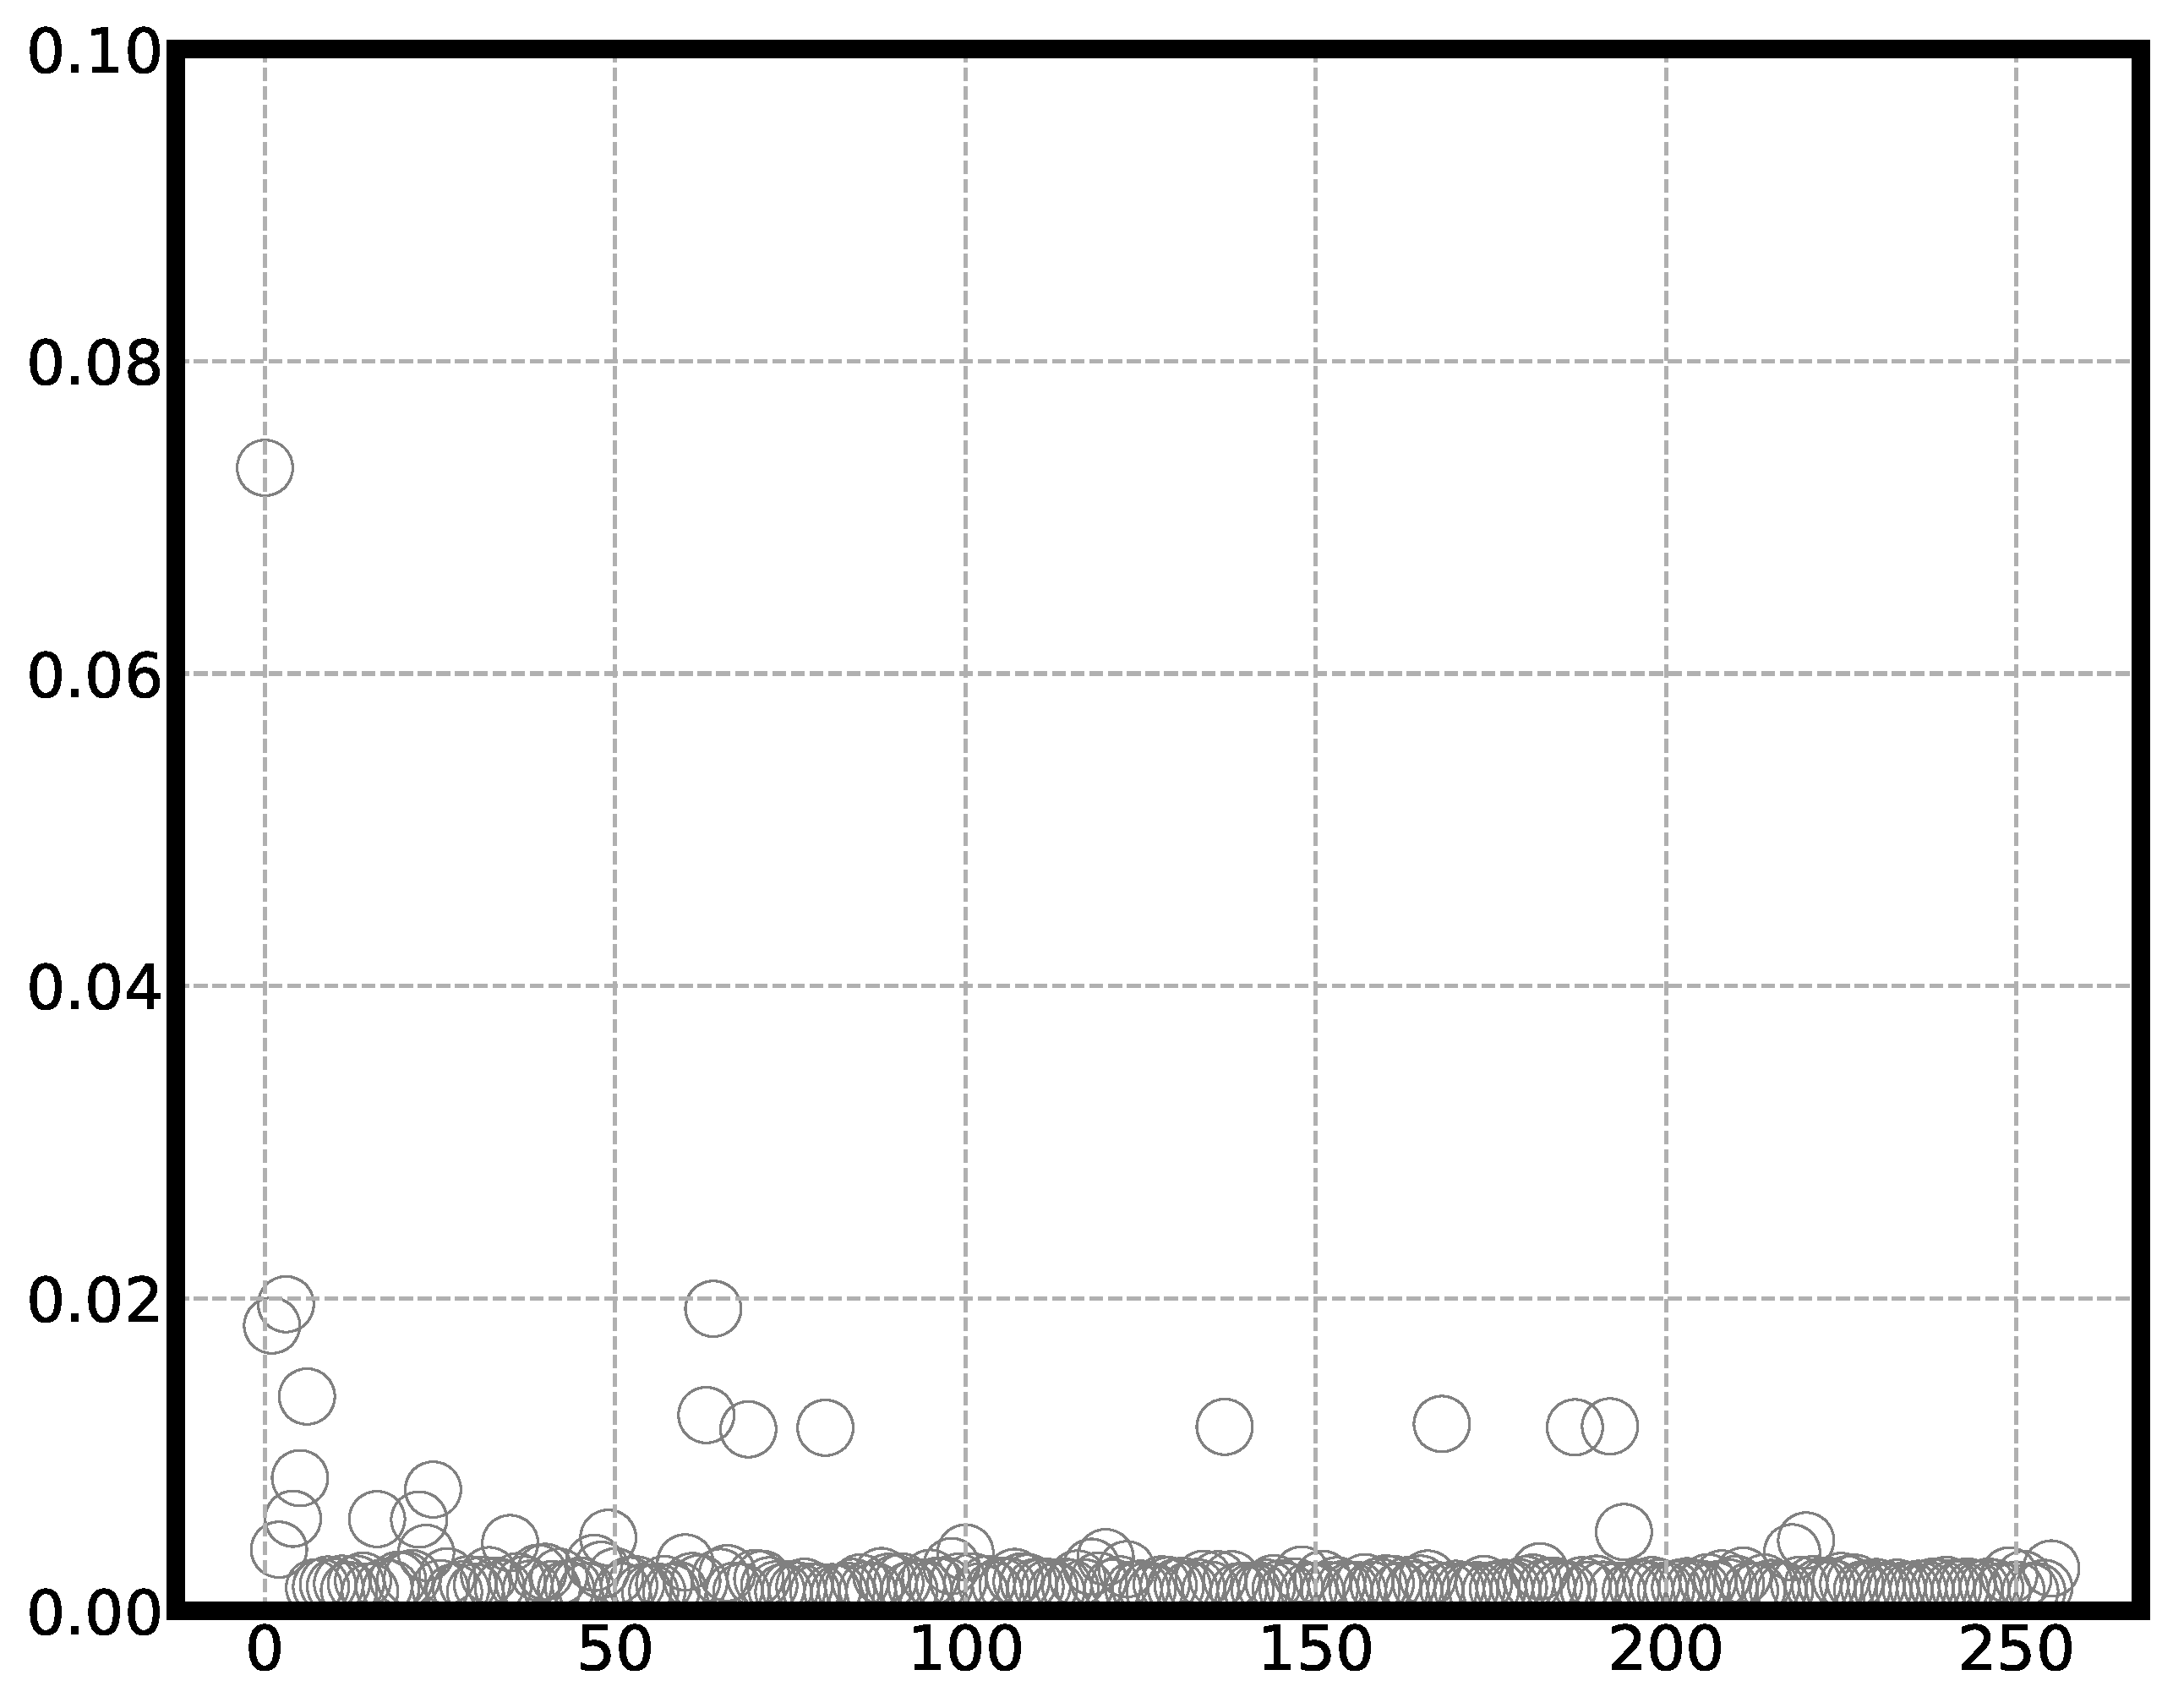
\includegraphics[width=\textwidth]{elem-payload.eps}
      \caption{}
      \label{fig:payload-elem}
    \end{subfigure}%
    ~% add desired spacing
    \begin{subfigure}[b]{0.35\textwidth}
      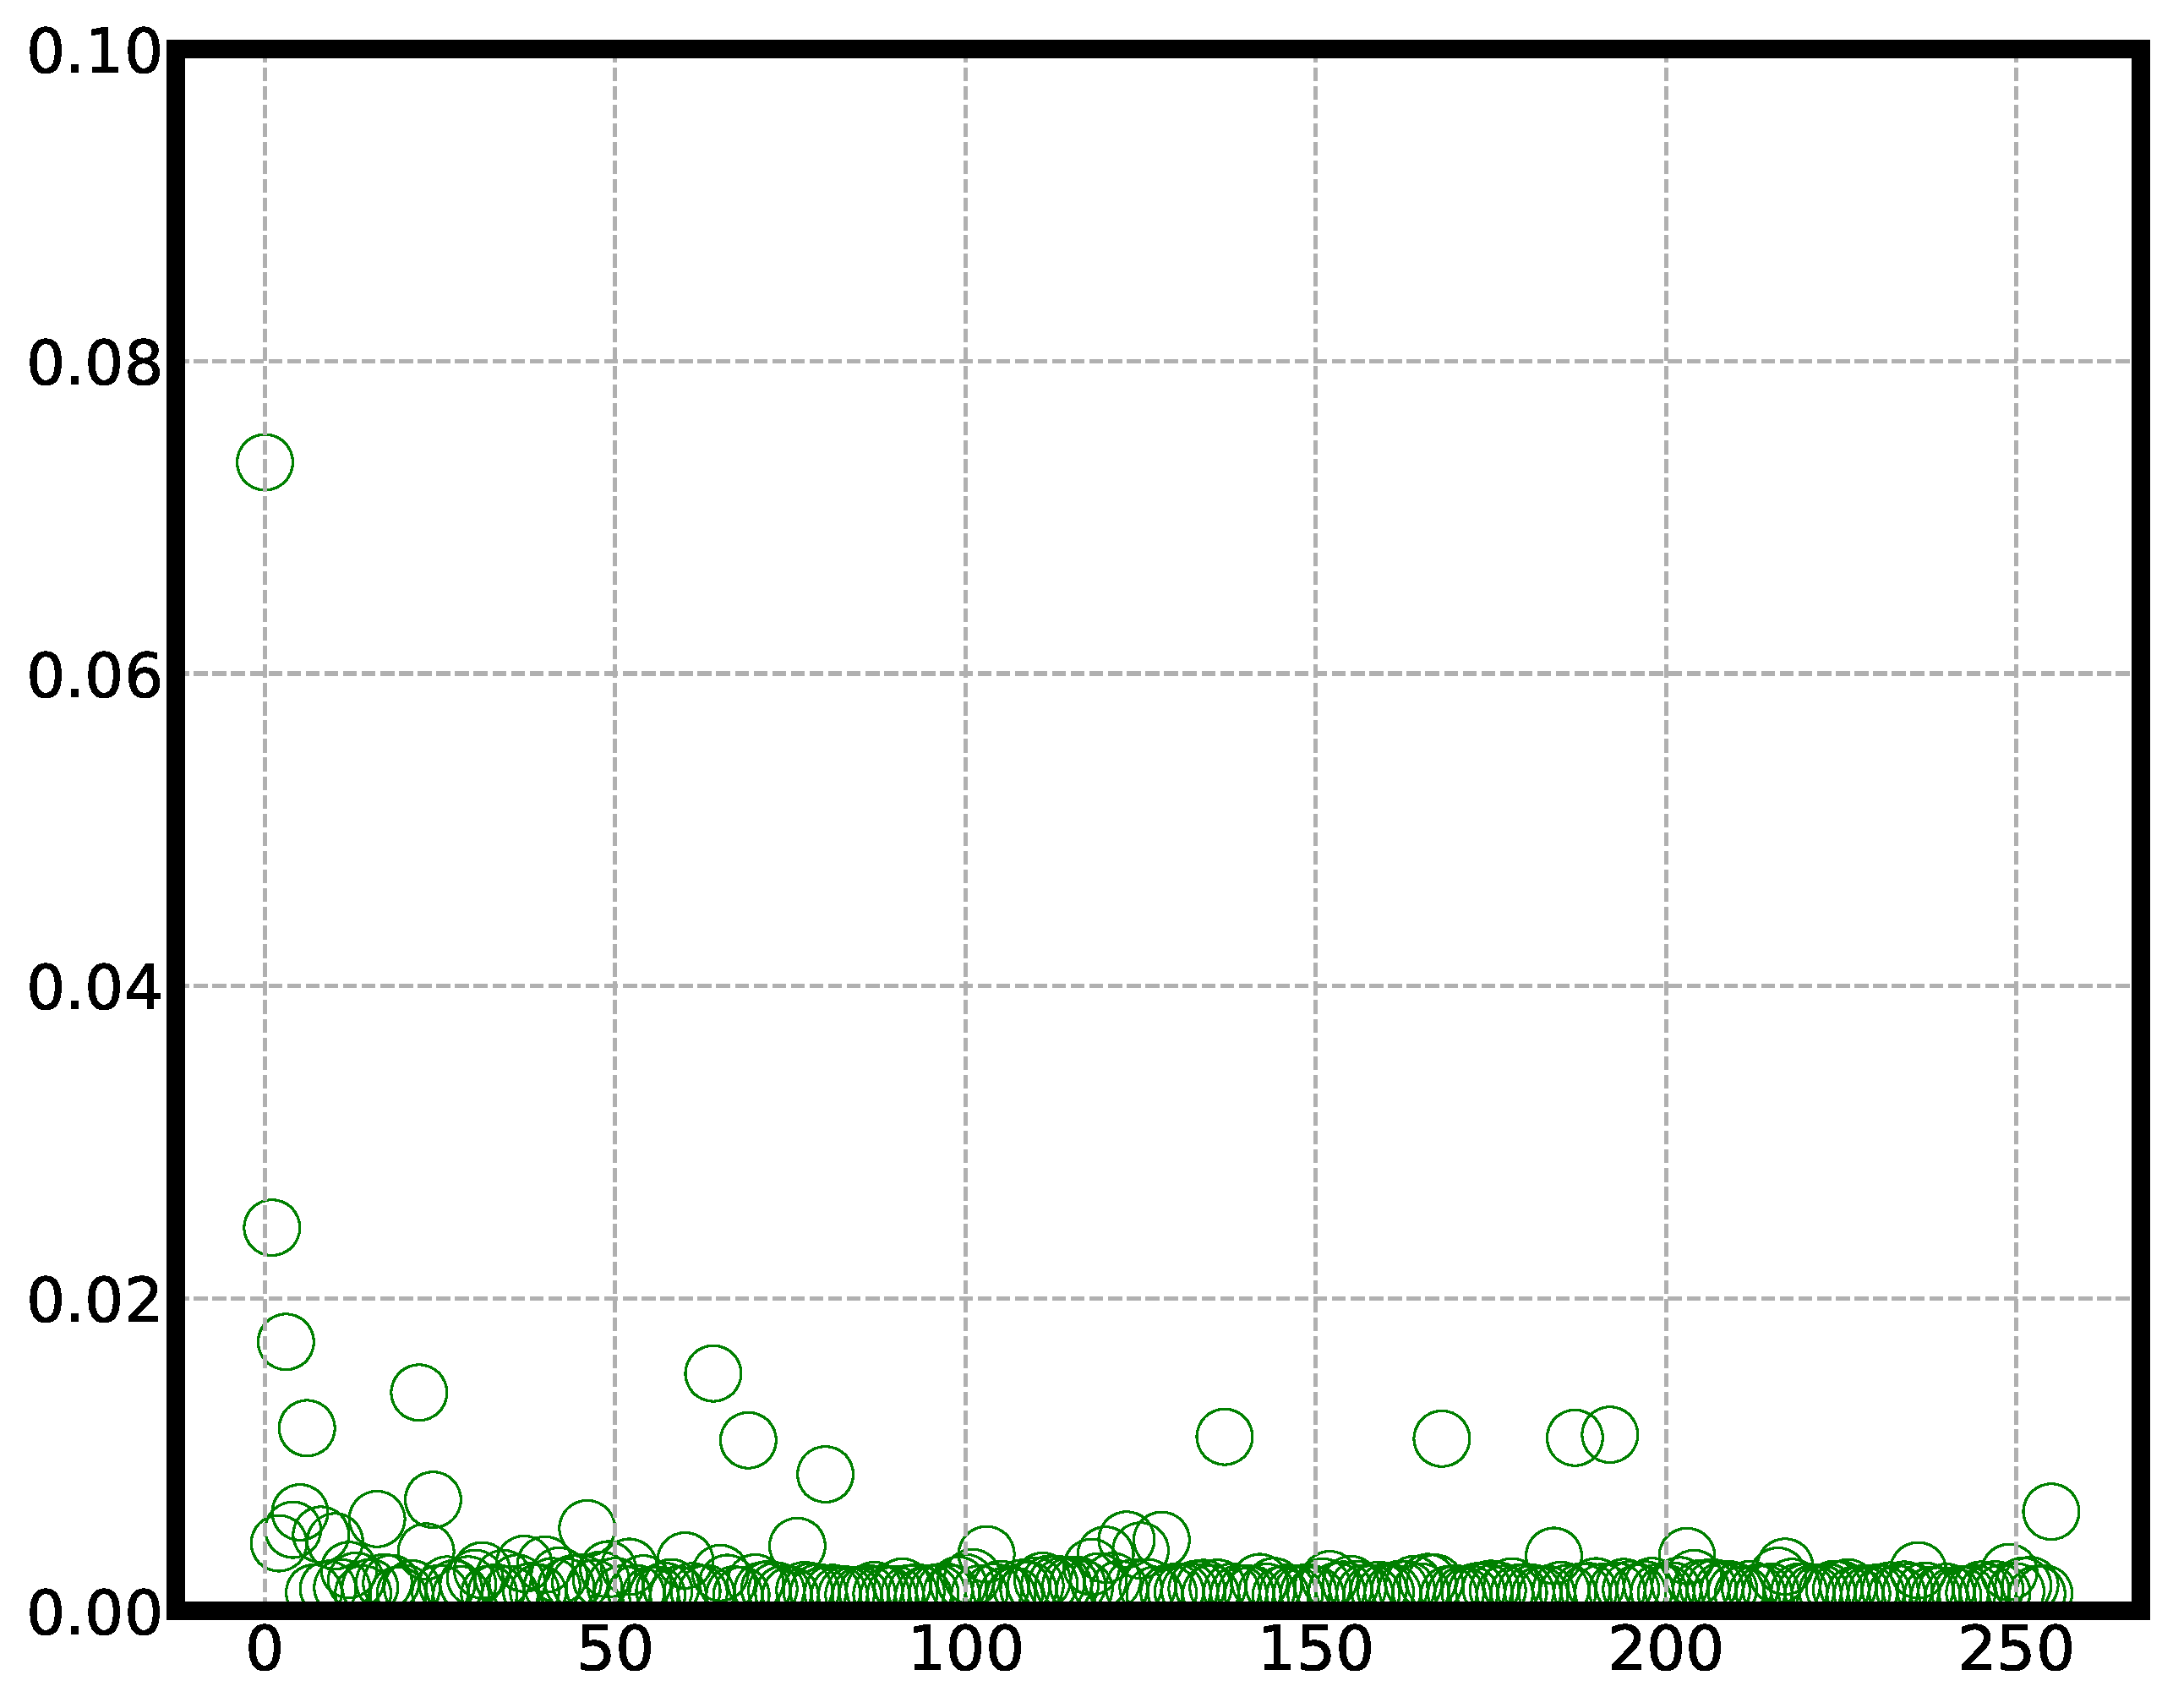
\includegraphics[width=\textwidth]{meituan-payload.eps}
      \caption{}
      \label{fig:payload-meituan}
    \end{subfigure}
    \\% line break
    \begin{subfigure}[b]{0.35\textwidth}
      \includegraphics[width=\textwidth]{jinritoutiao-payload.eps}
      \caption{}
      \label{fig:payload-jinritoutiao}
    \end{subfigure}%
    ~% add desired spacing
    \begin{subfigure}[b]{0.35\textwidth}
      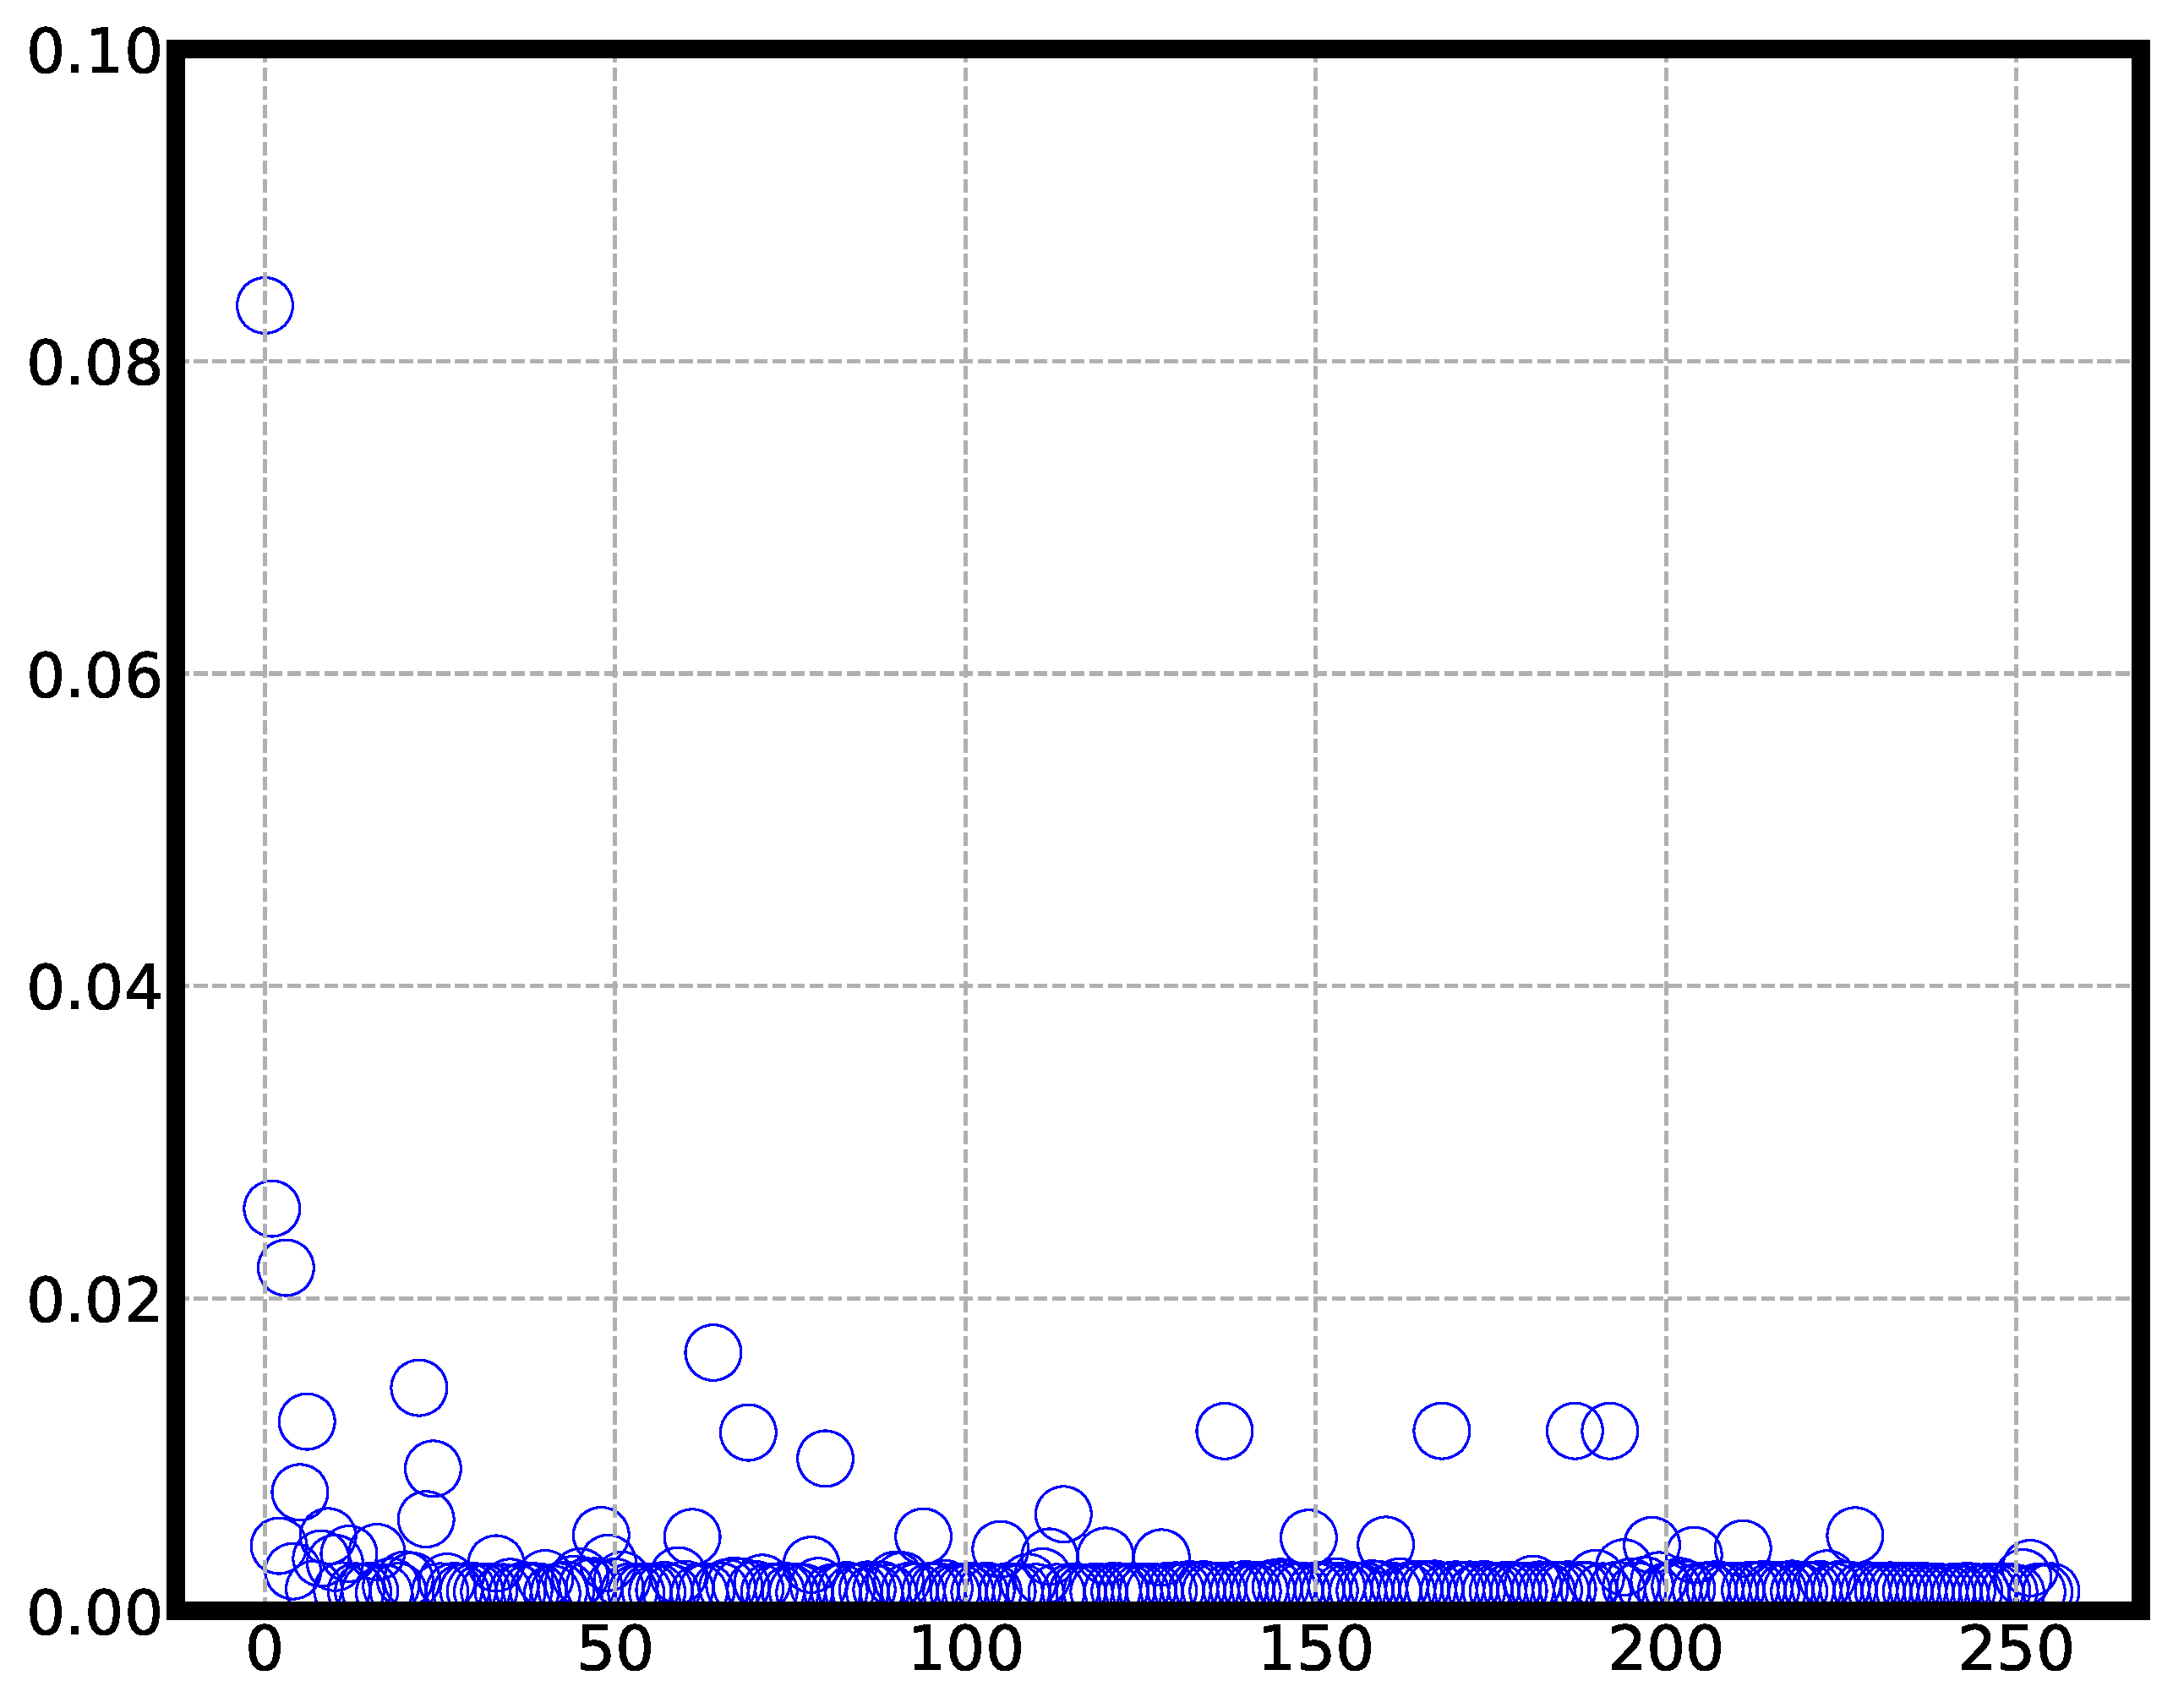
\includegraphics[width=\textwidth]{cloudmusic-payload.eps}
      \caption{}
      \label{fig:payload-netease-cloud-music}
    \end{subfigure}
    \bicaption{负载特征。(a) 饿了么,(b) 美团,(c) 今日头条,(d) 网易云音乐。}{PAYLOAD.(a)Ele , (b)Meituan , (c)Jinritoutiao , (d)Netease-cloud-music.}
    \label{fig:payload-eda}
\end{figure}

%-------------------------------------------------------------------------
\subsubsection{parameter部分}
形成CT视图。

\begin{table}[!htbp]
    \bicaption{内容类型。}{Content Type.}
    \label{tab:content-type}
    \centering
    \footnotesize% fontsize
    \setlength{\tabcolsep}{4pt}% column separation
    \renewcommand{\arraystretch}{1.2}%row space
    \resizebox{\columnwidth}{!}{
        \begin{tabular}{rccc}
        \textbf{取值} & \textbf{描述} & \textbf{DTLS-OJ} & \textbf{参考}\\
        \hline
        0-19 & Unassigned (Requires coordination; see [RFC7983]) & & [RFC5764][RFC7983]\\
        20 & change\_cipher\_spec & Y & [RFC8446]\\
        21 & alert & Y & [RFC8446]\\
        22 & handshake & Y & [RFC8446]\\
        23 & application\_data & Y & [RFC8446]\\
        24 & heartbeat & Y & [RFC6520]\\
        25 & tls12\_cid (TEMPORARY - registered 2019-07-02, expires 2020-07-02) & Y & [draft-ietf-tls-dtls-connection-id]\\
        26-63 & Unassigned & & \\
        64-255 & Unassigned (Requires coordination; see [RFC7983]) & & [RFC5764][RFC7983]\\
        \hline
        \end{tabular}    
    
    }

\end{table}



\begin{figure}[!htbp]
    \centering
    \begin{subfigure}[b]{0.35\textwidth}
      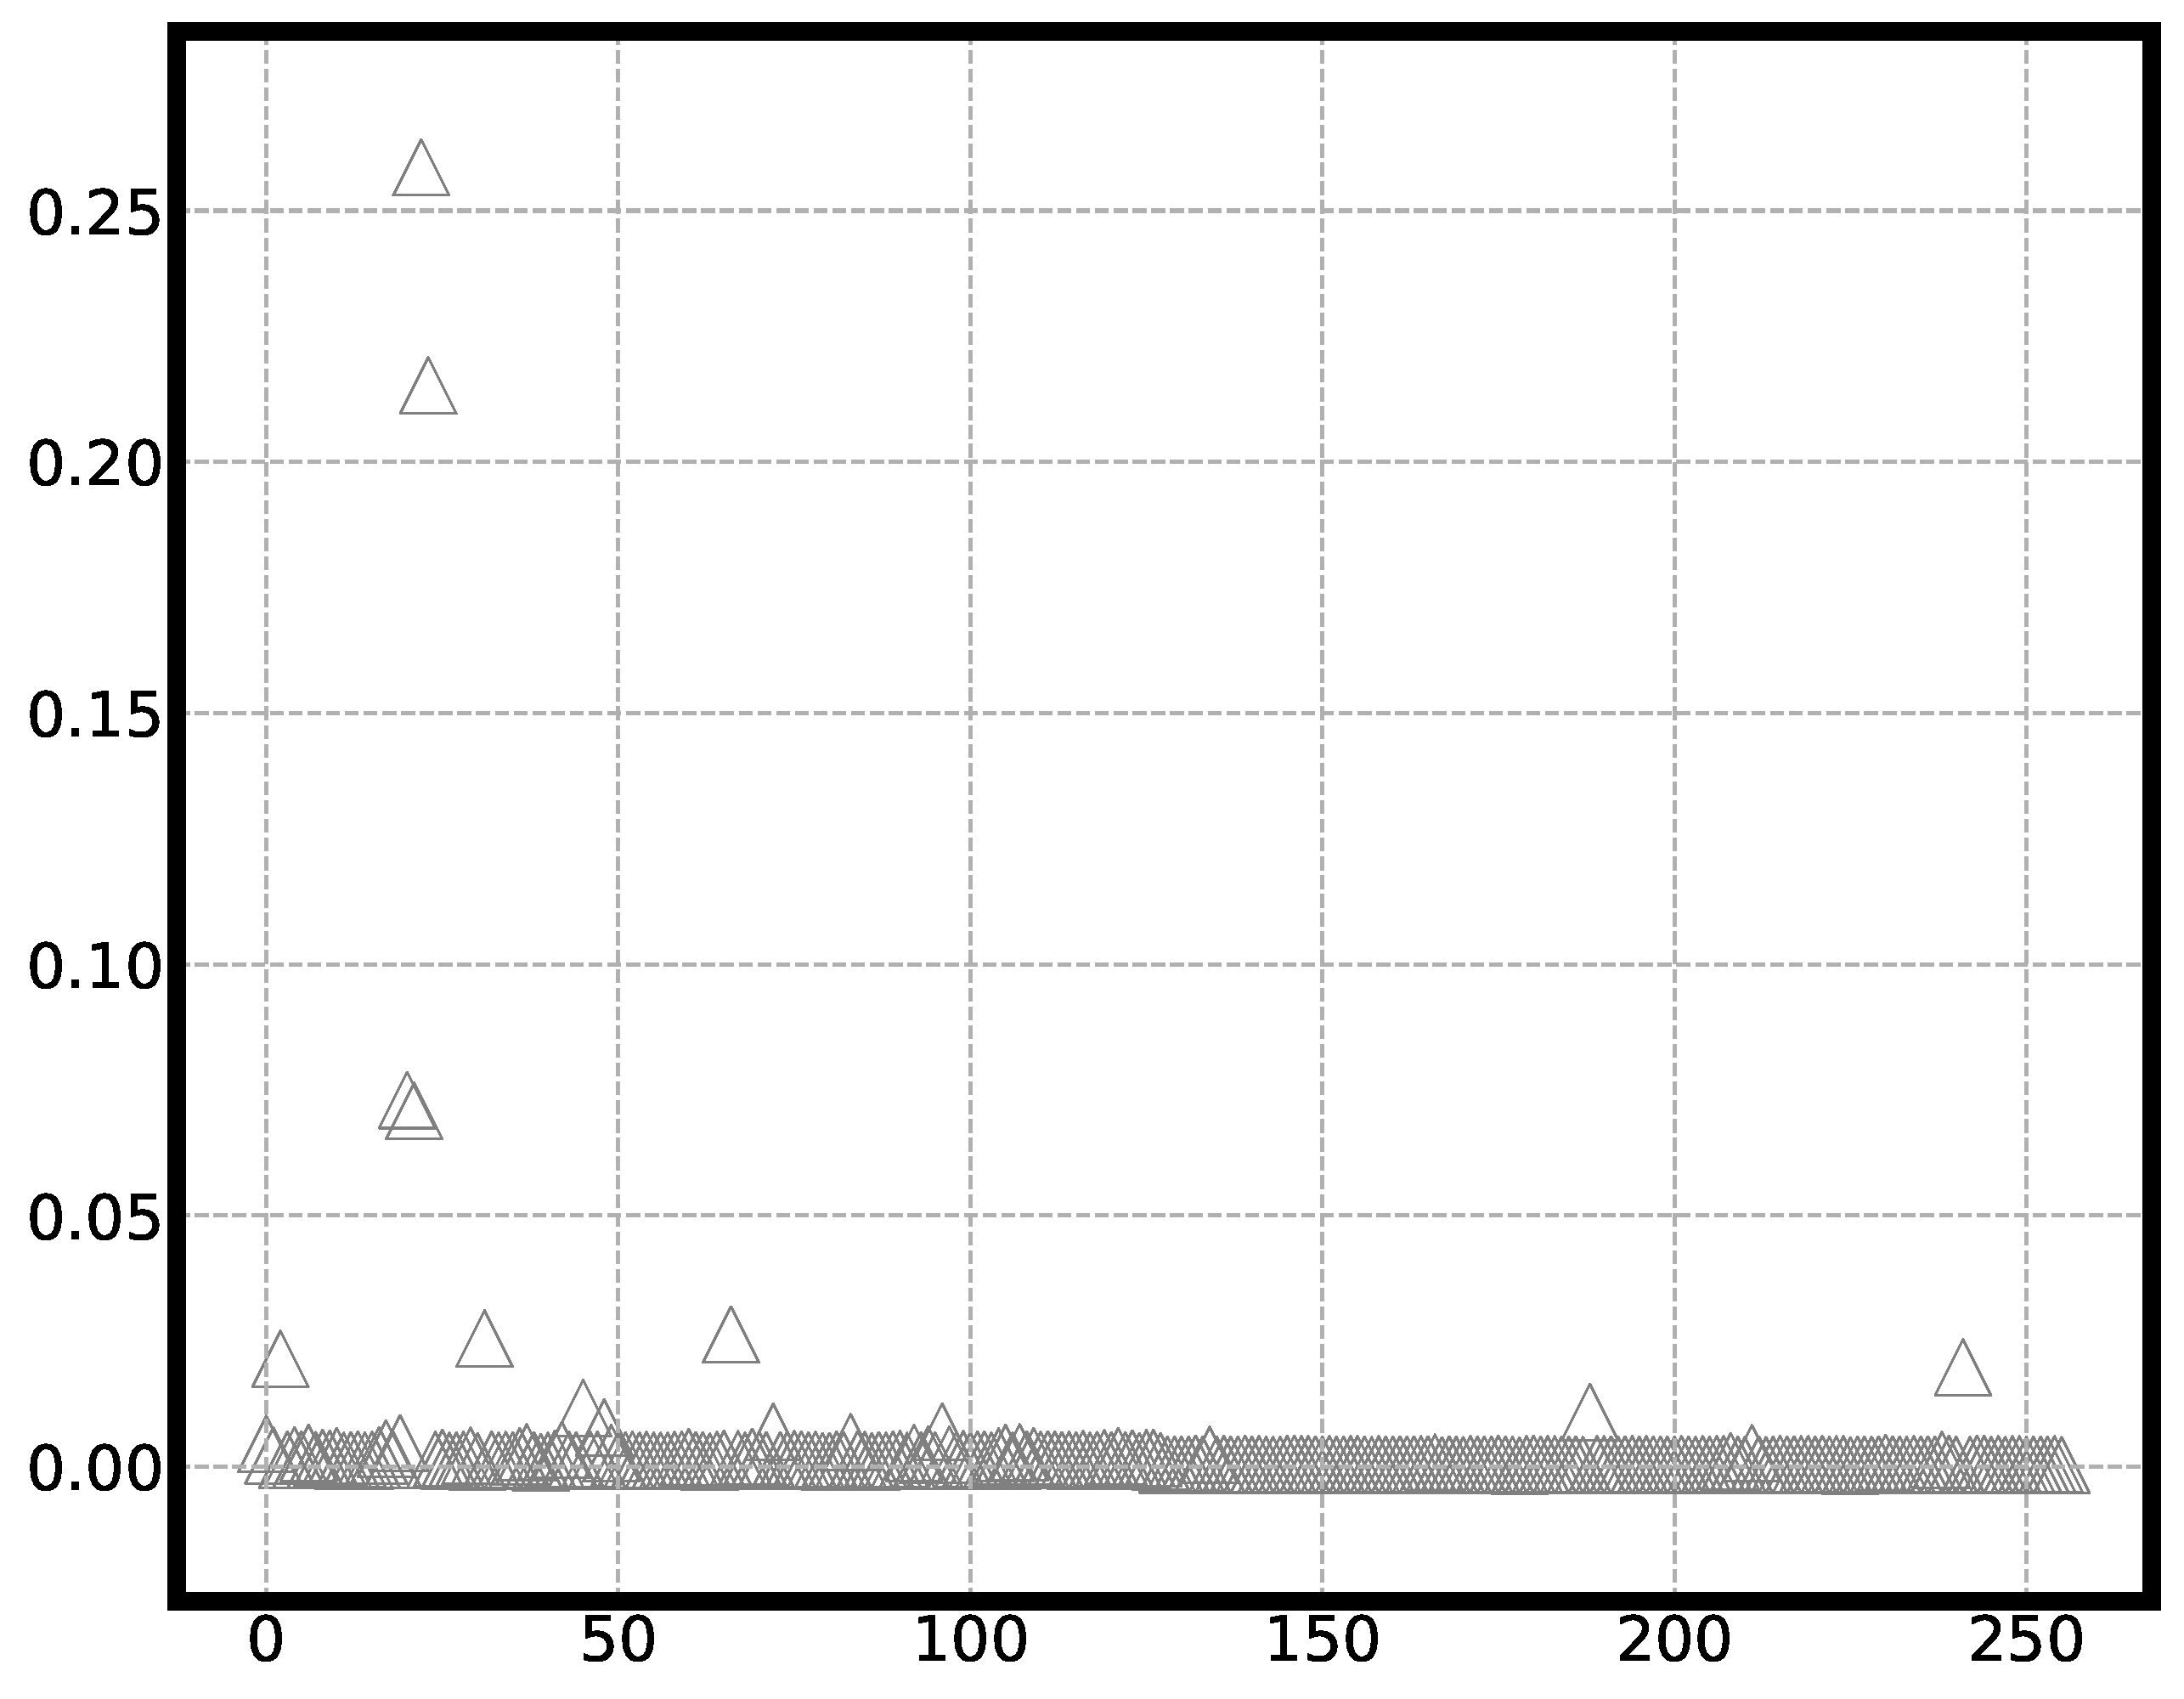
\includegraphics[width=\textwidth]{elem-contenttype.eps}
      \caption{}
      \label{fig:oaspl_a}
    \end{subfigure}%
    ~% add desired spacing
    \begin{subfigure}[b]{0.35\textwidth}
      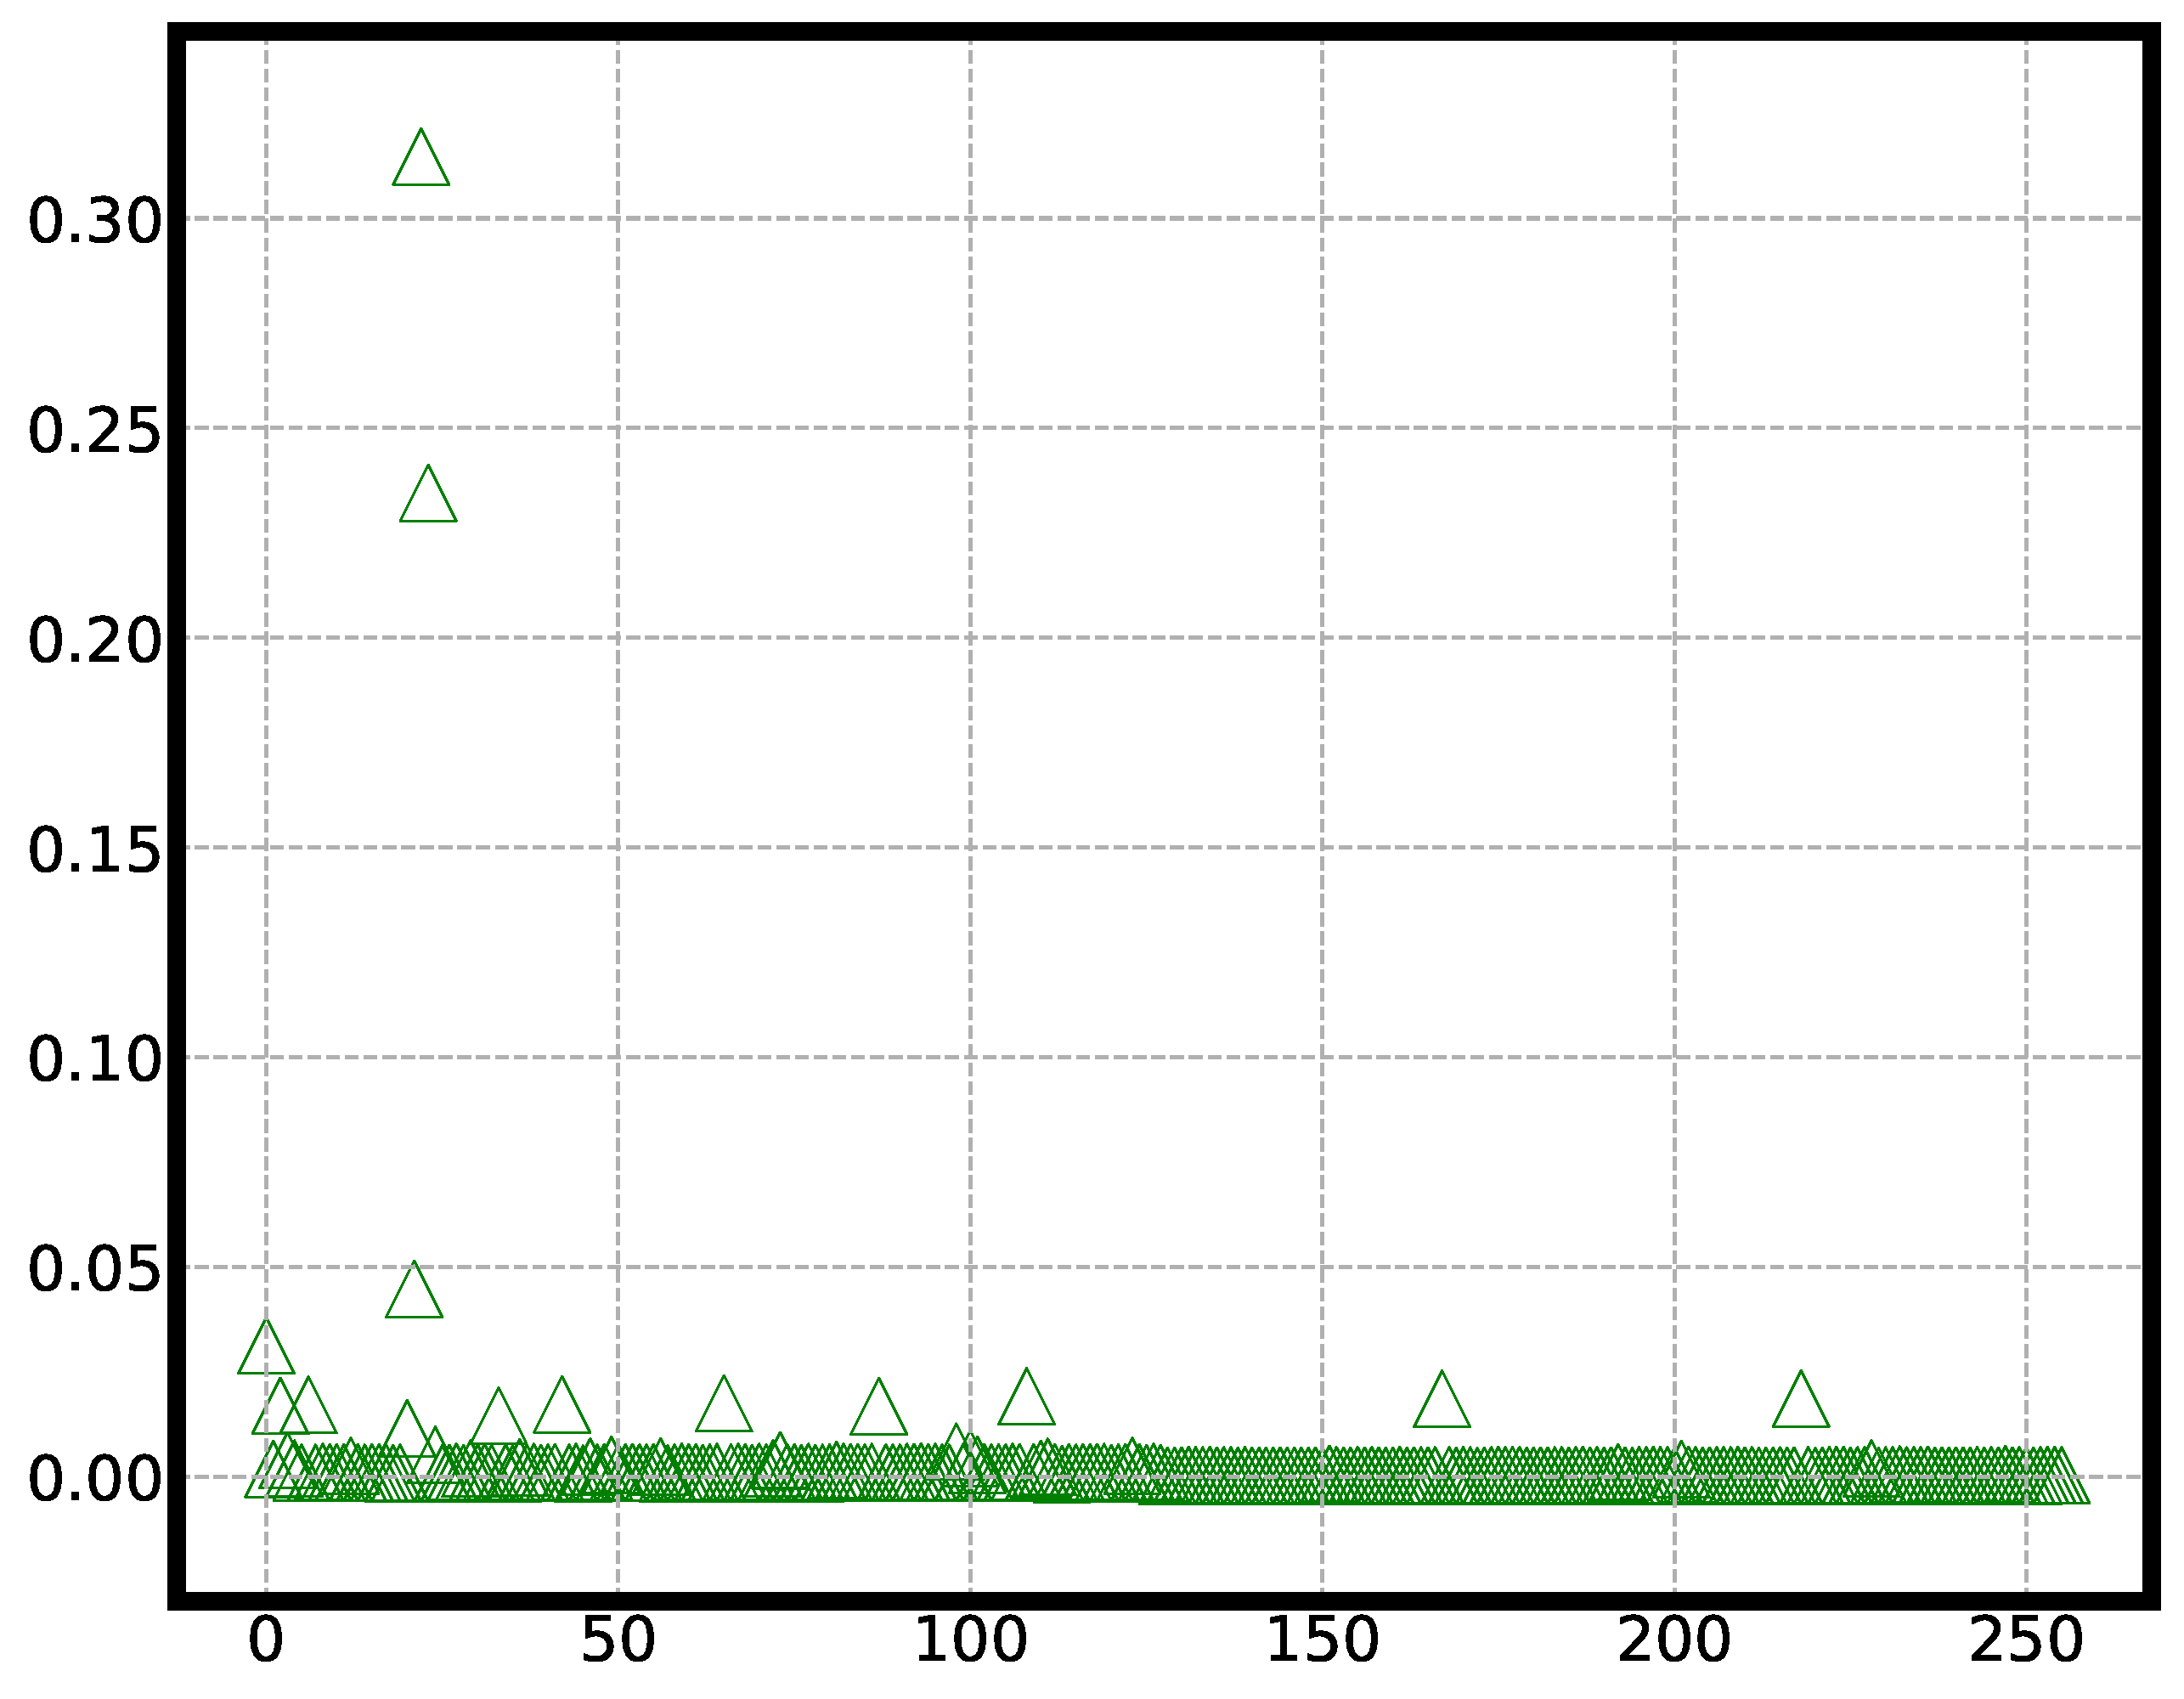
\includegraphics[width=\textwidth]{meituan-contenttype.eps}
      \caption{}
      \label{fig:oaspl_b}
    \end{subfigure}
    \\% line break
    \begin{subfigure}[b]{0.35\textwidth}
      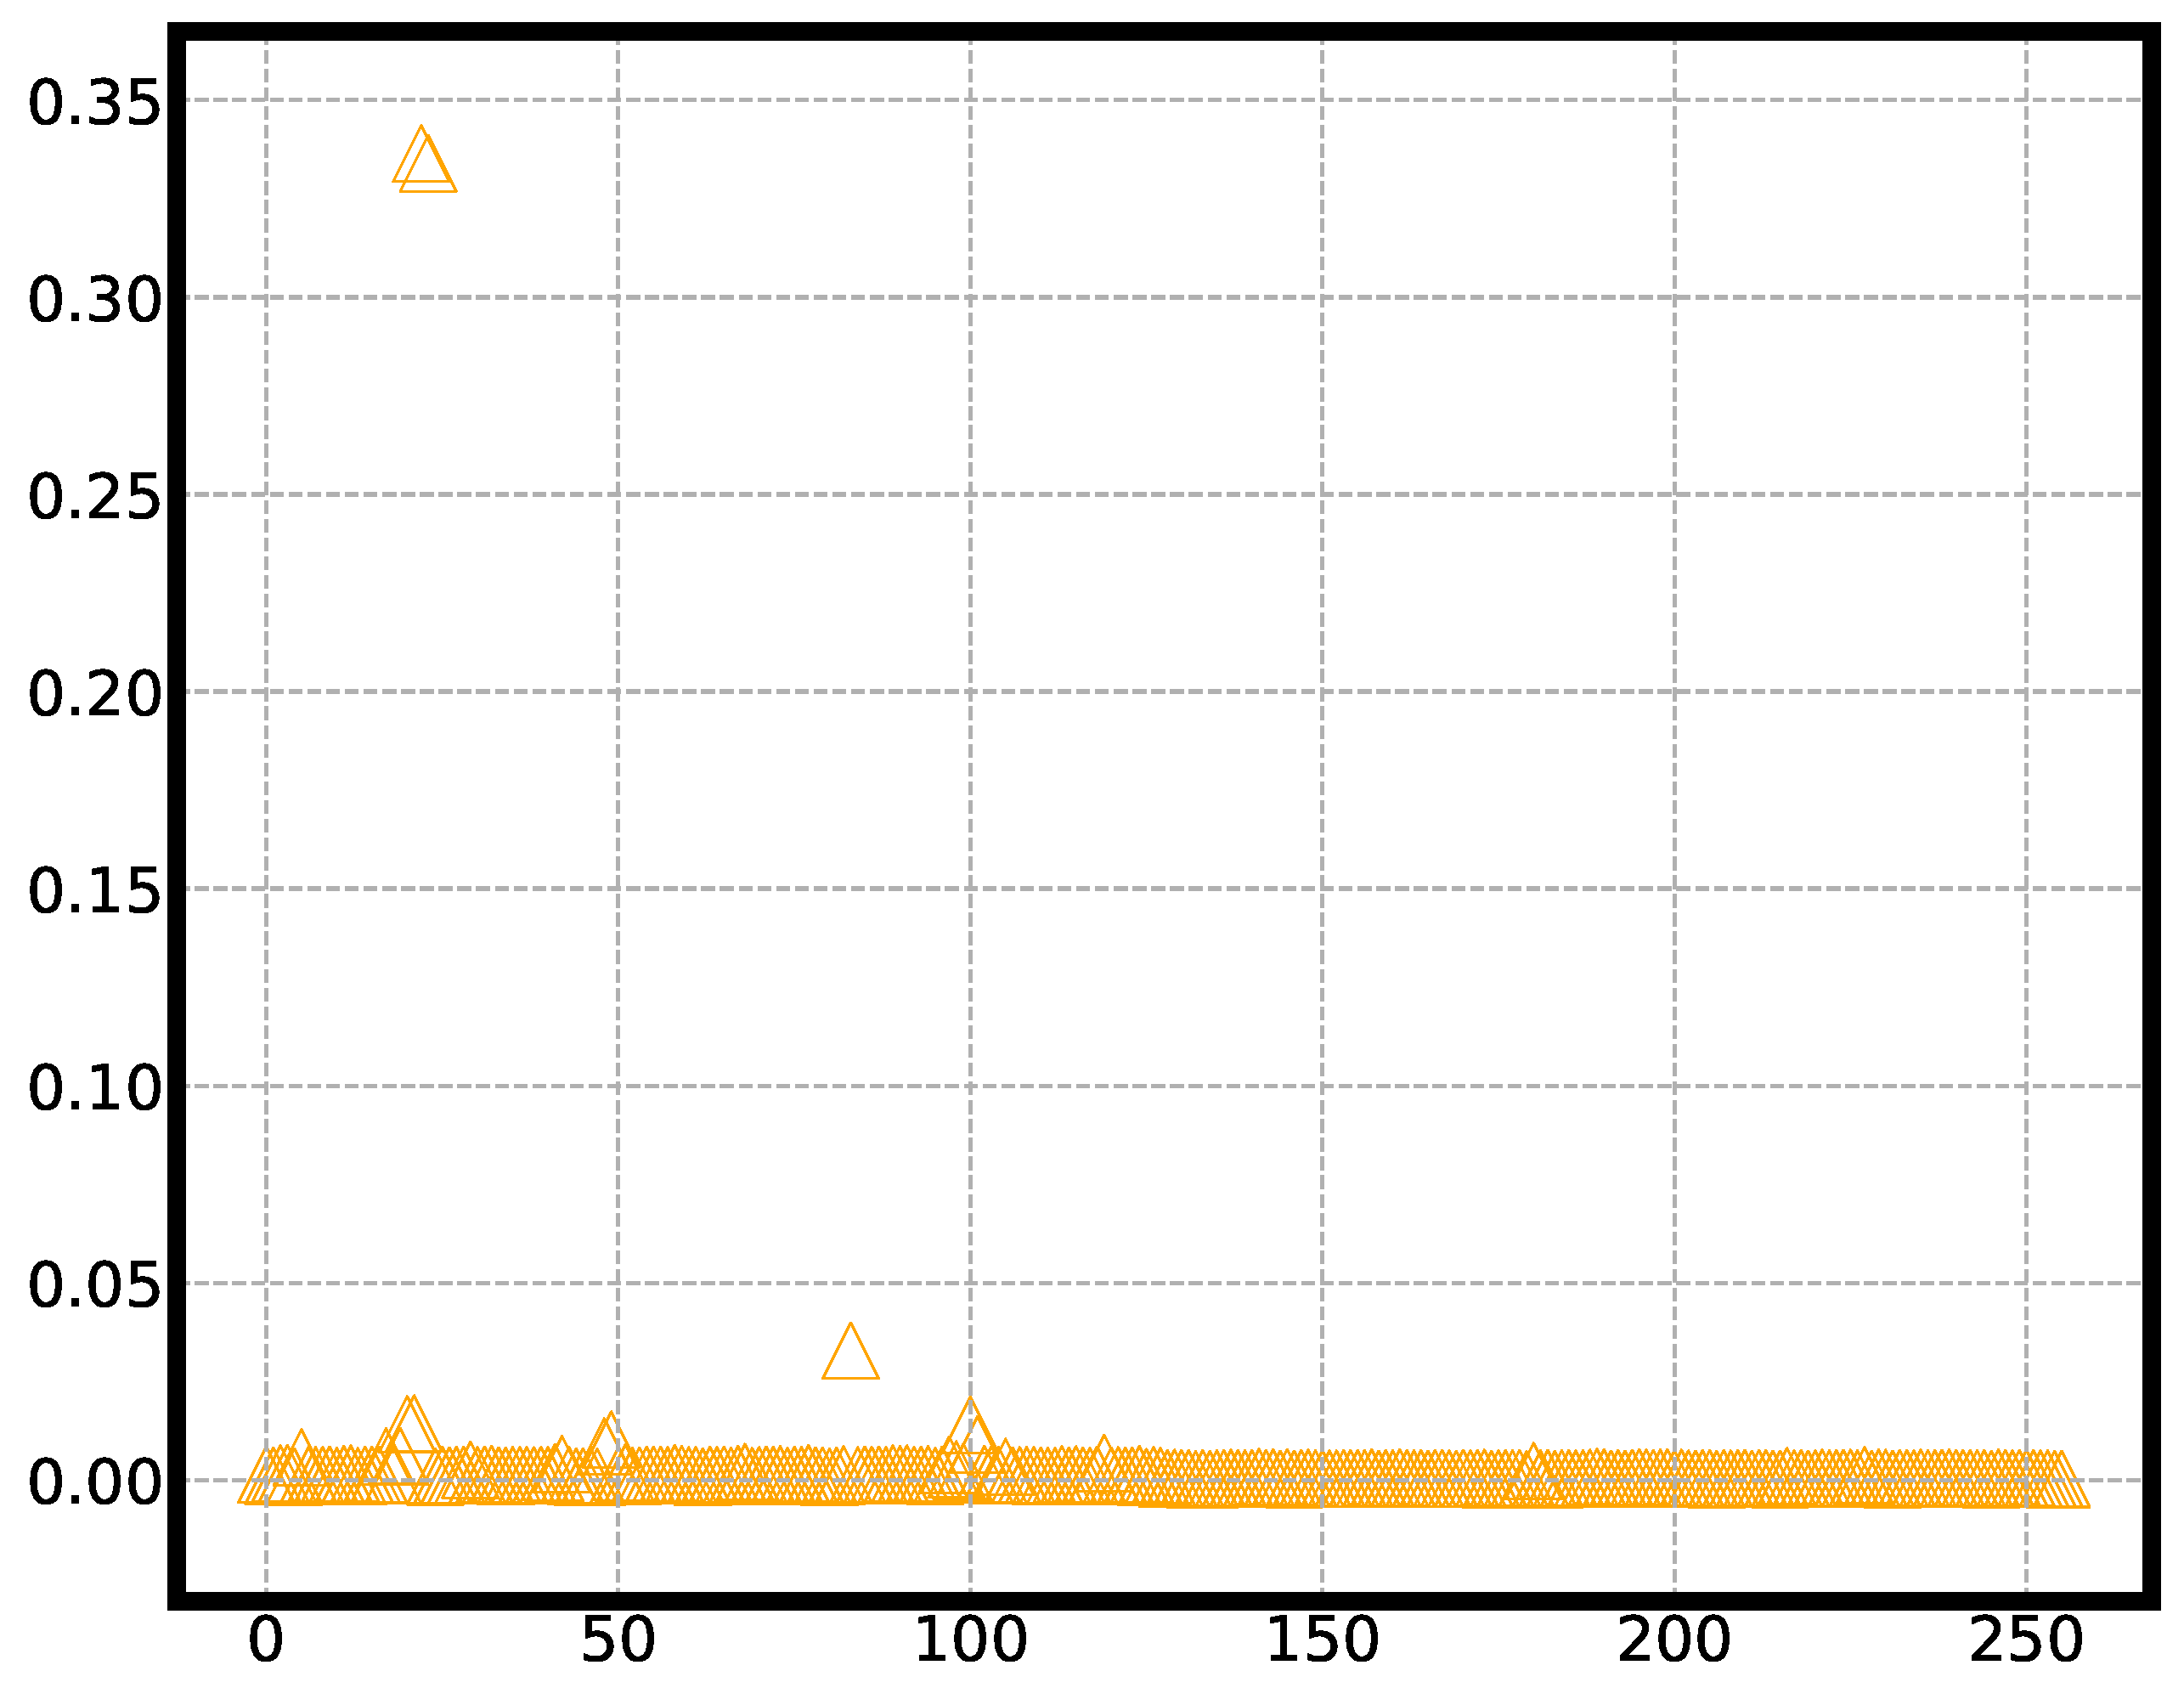
\includegraphics[width=\textwidth]{jinritoutiao-contenttype.eps}
      \caption{}
      \label{fig:oaspl_c}
    \end{subfigure}%
    ~% add desired spacing
    \begin{subfigure}[b]{0.35\textwidth}
      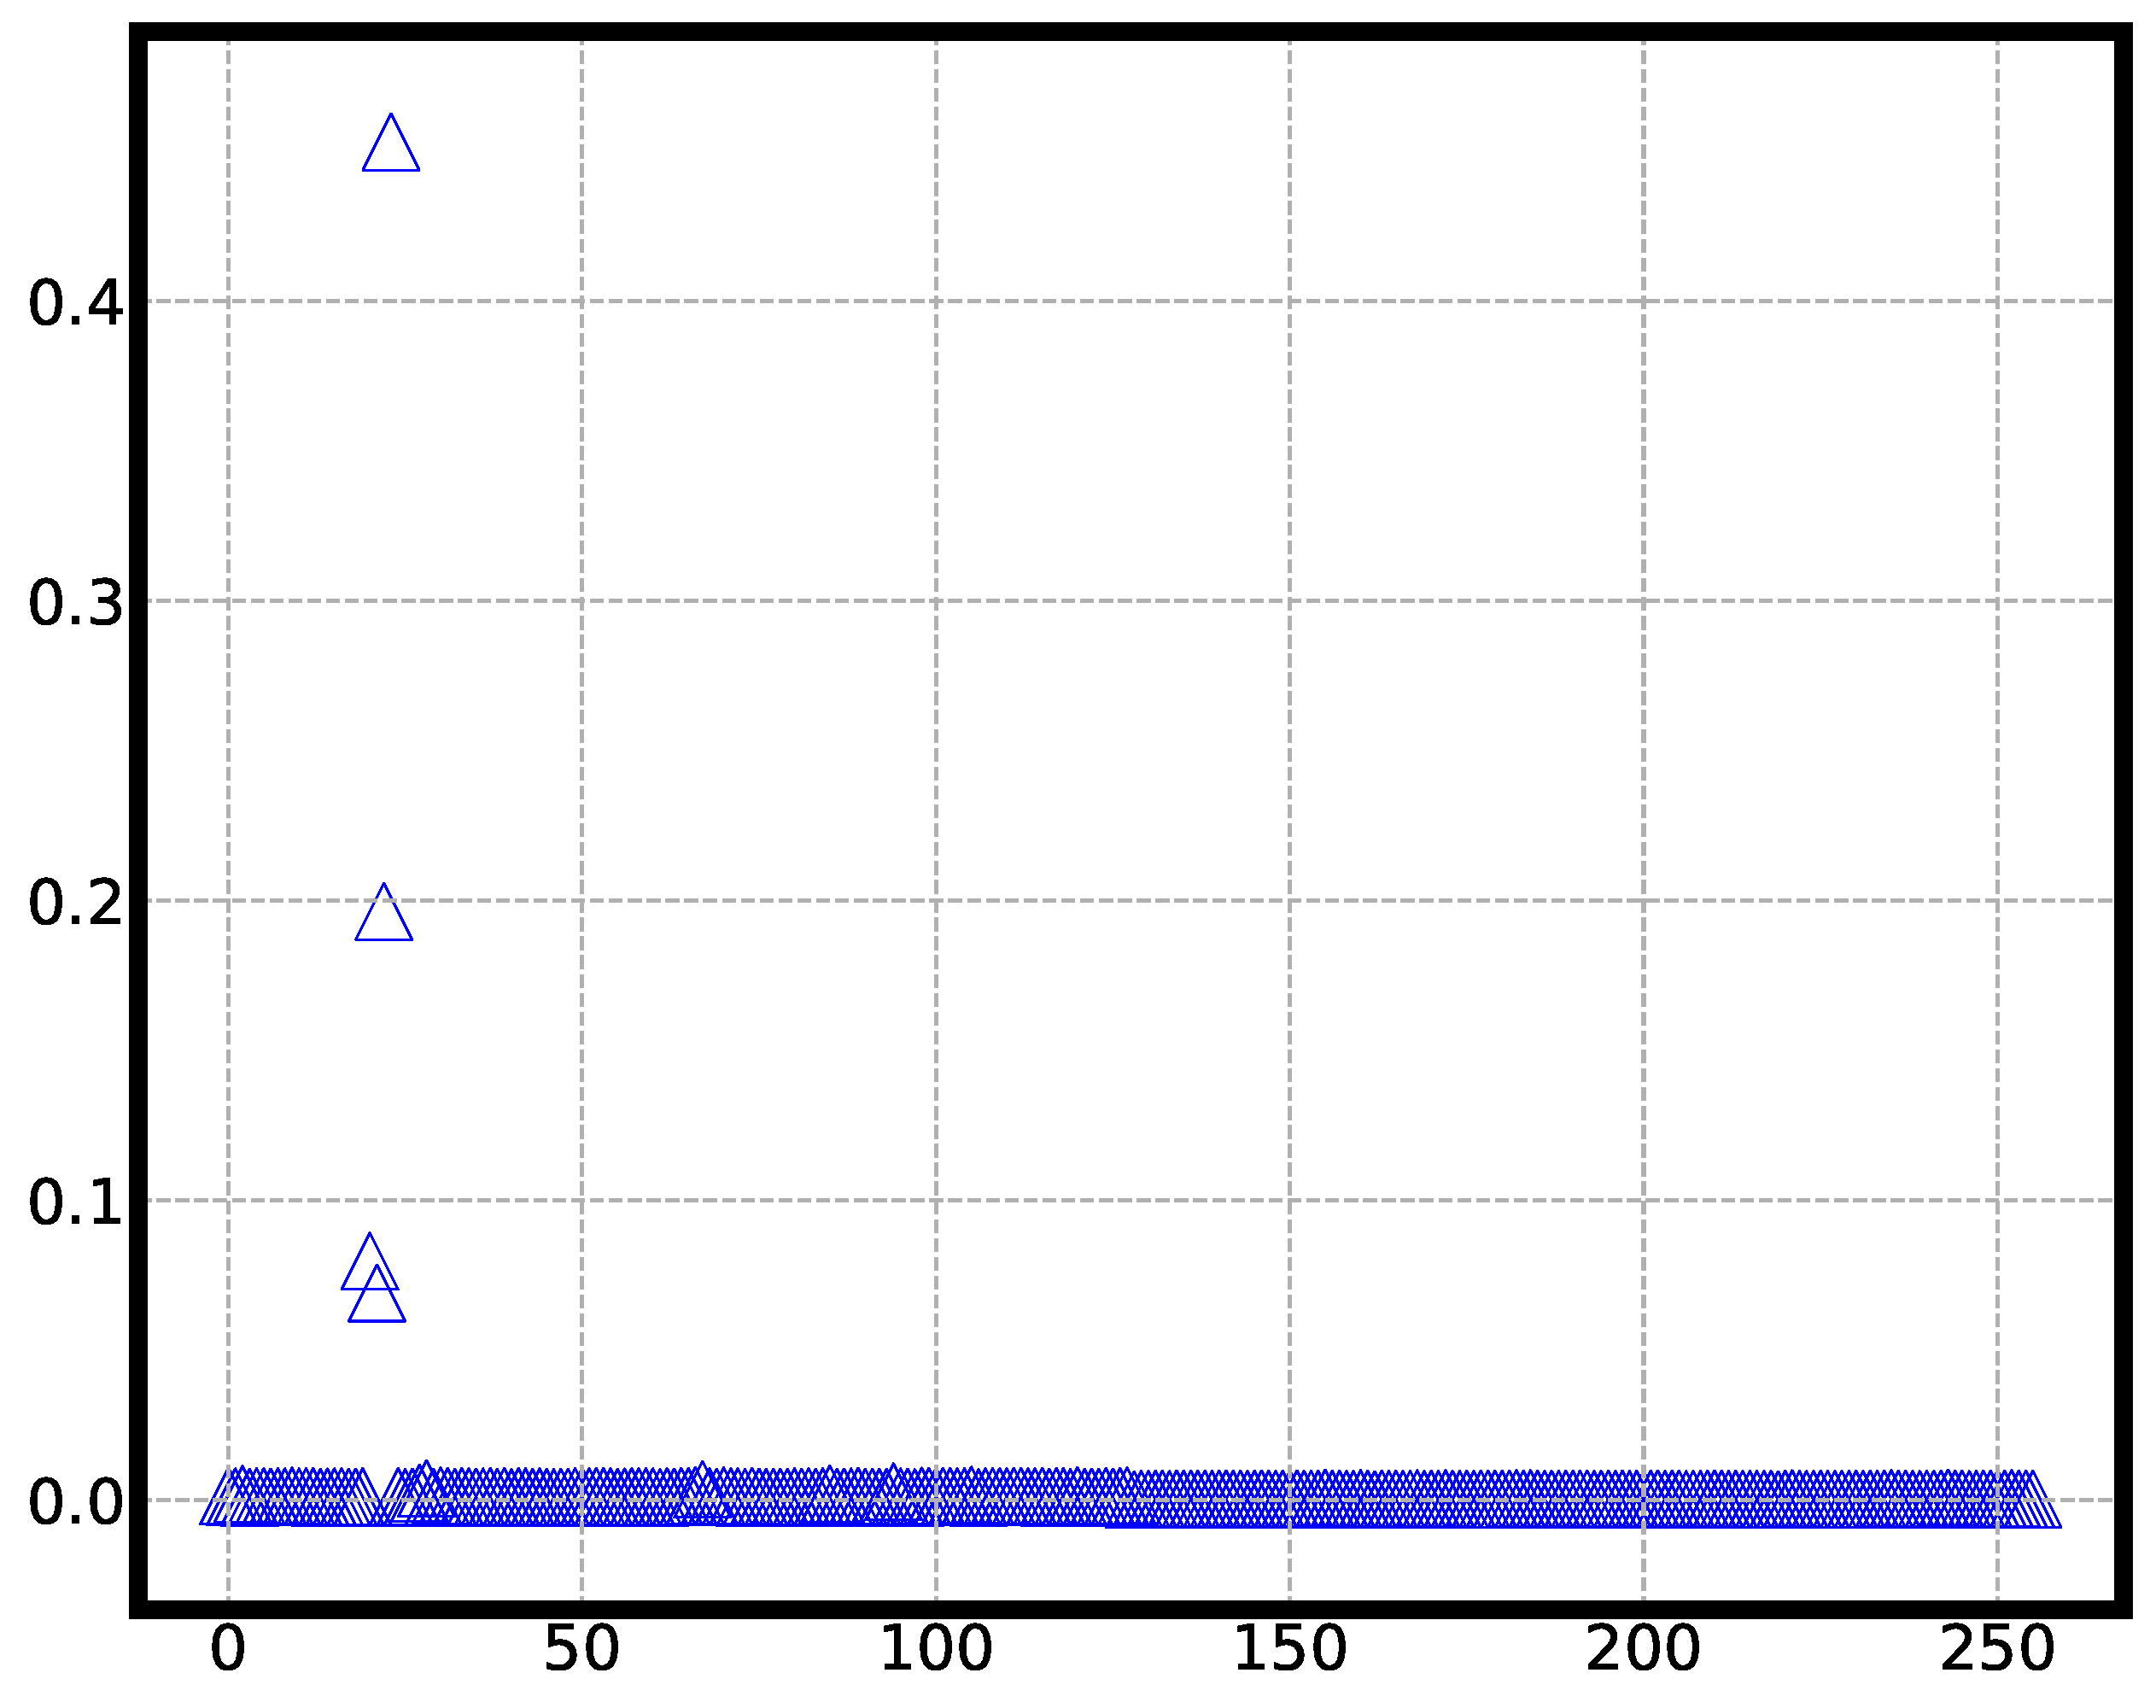
\includegraphics[width=\textwidth]{cloudmusic-contenttype.eps}
      \caption{}
      \label{fig:oaspl_d}
    \end{subfigure}
    \bicaption{内容类型特征。(a) 饿了么,(b) 美团,(c) 今日头条,(d) 网易云音乐。}{PAYLOAD.(a)Ele , (b)Meituan , (c)Jinritoutiao , (d)Netease-cloud-music.}
    \label{fig:content-type-eda}
\end{figure}


%-----------------------------------------------------------------------
\subsubsection{packet size部分}
形成PS视图。
\begin{figure}[!htbp]
    \centering
    \begin{subfigure}[b]{0.35\textwidth}
      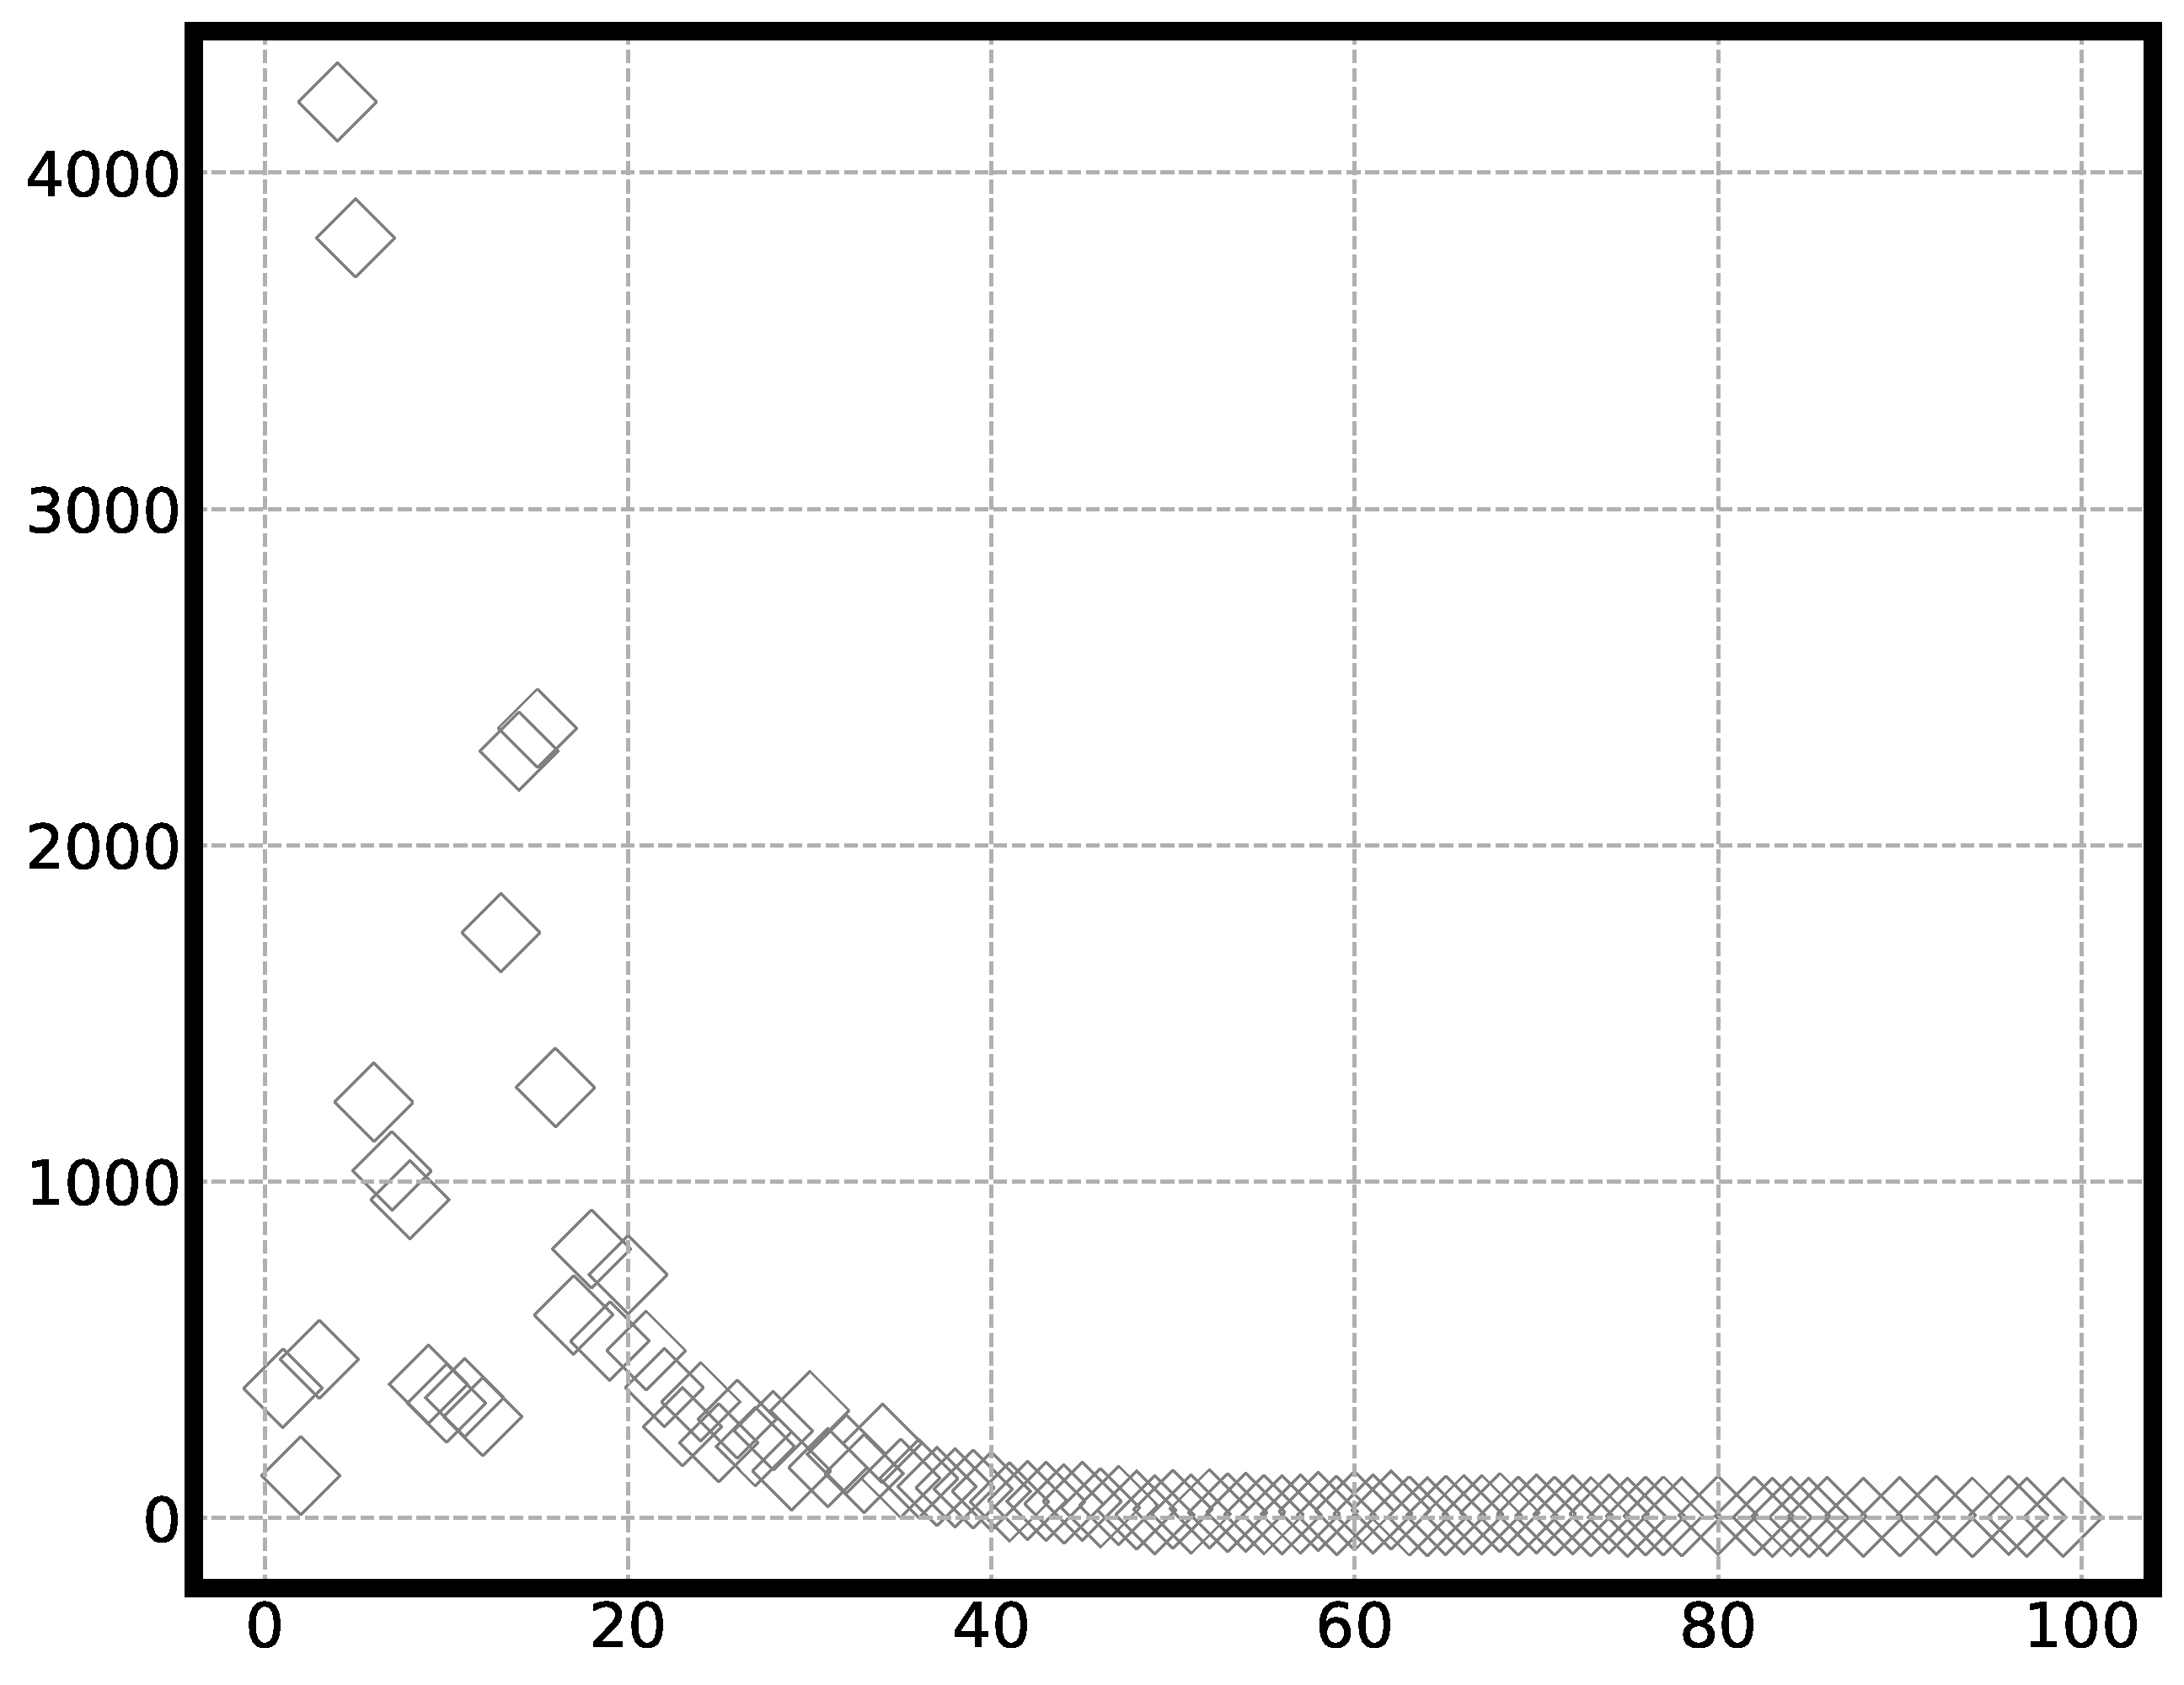
\includegraphics[width=\textwidth]{elem-count.eps}
      \caption{}
      \label{fig:packet-size-ele}
    \end{subfigure}%
    ~% add desired spacing
    \begin{subfigure}[b]{0.35\textwidth}
      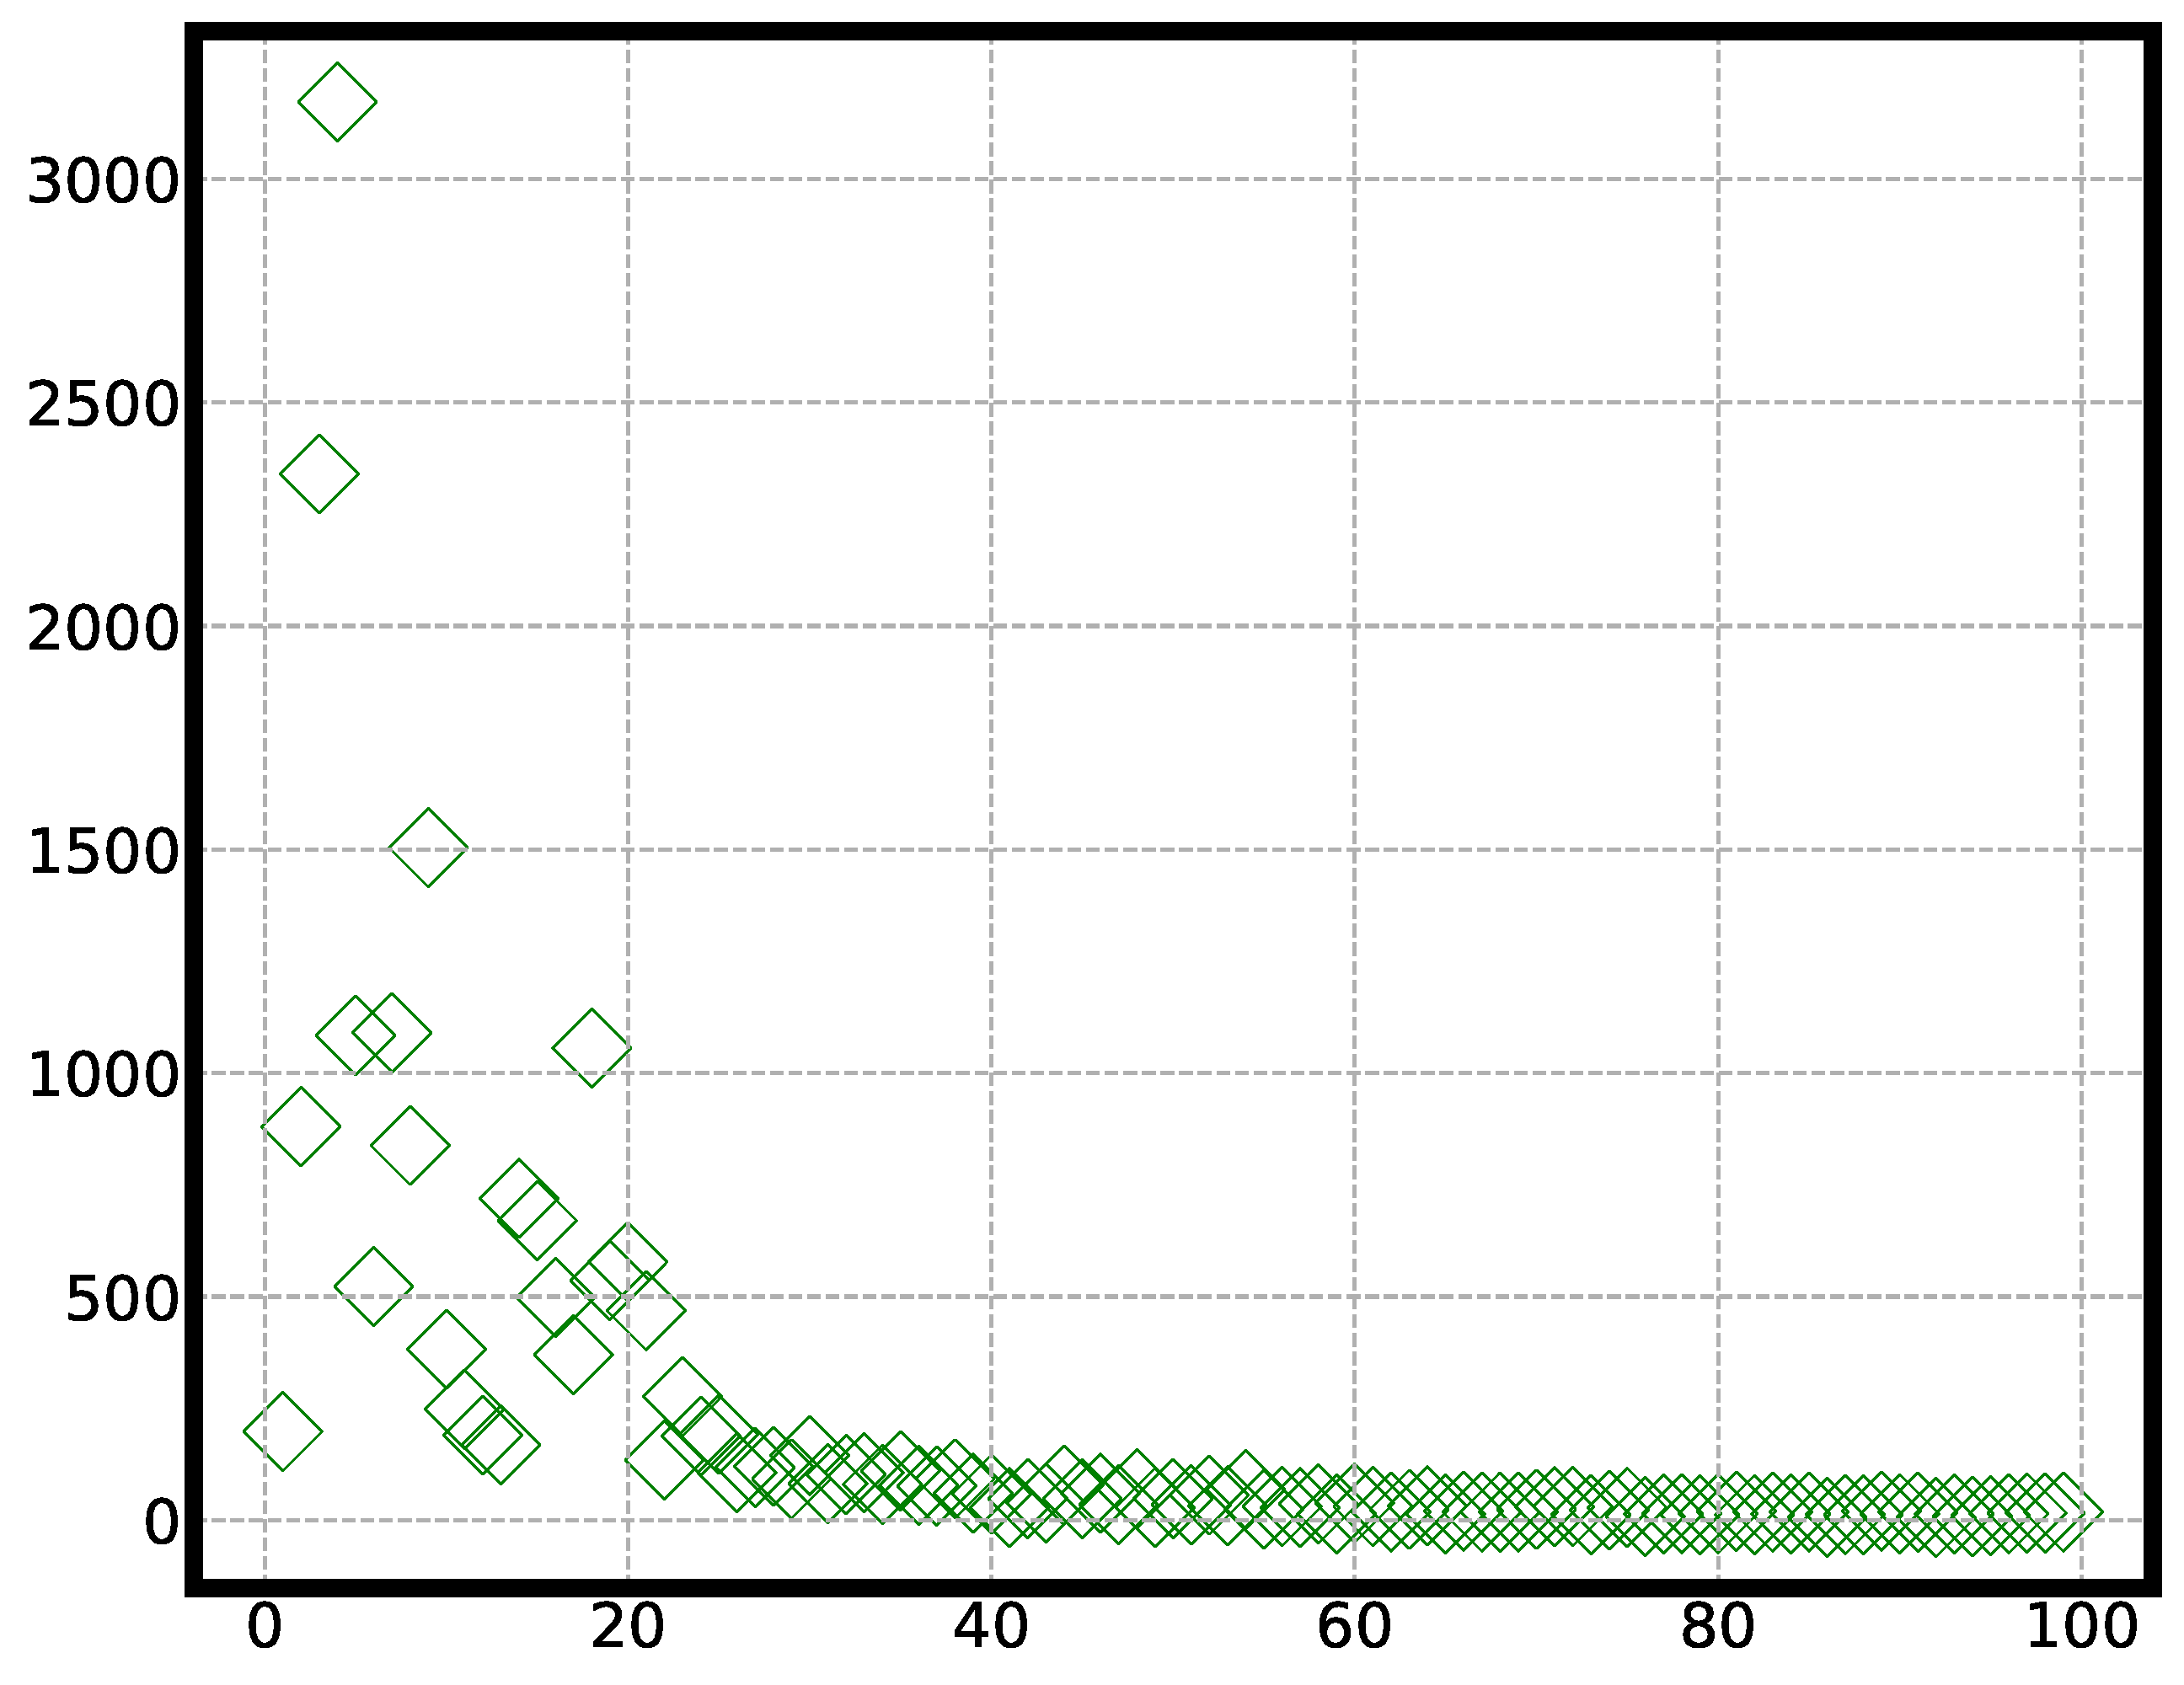
\includegraphics[width=\textwidth]{meituan-count.eps}
      \caption{}
      \label{fig:packet-size-meituan}
    \end{subfigure}
    \\% line break
    \begin{subfigure}[b]{0.35\textwidth}
      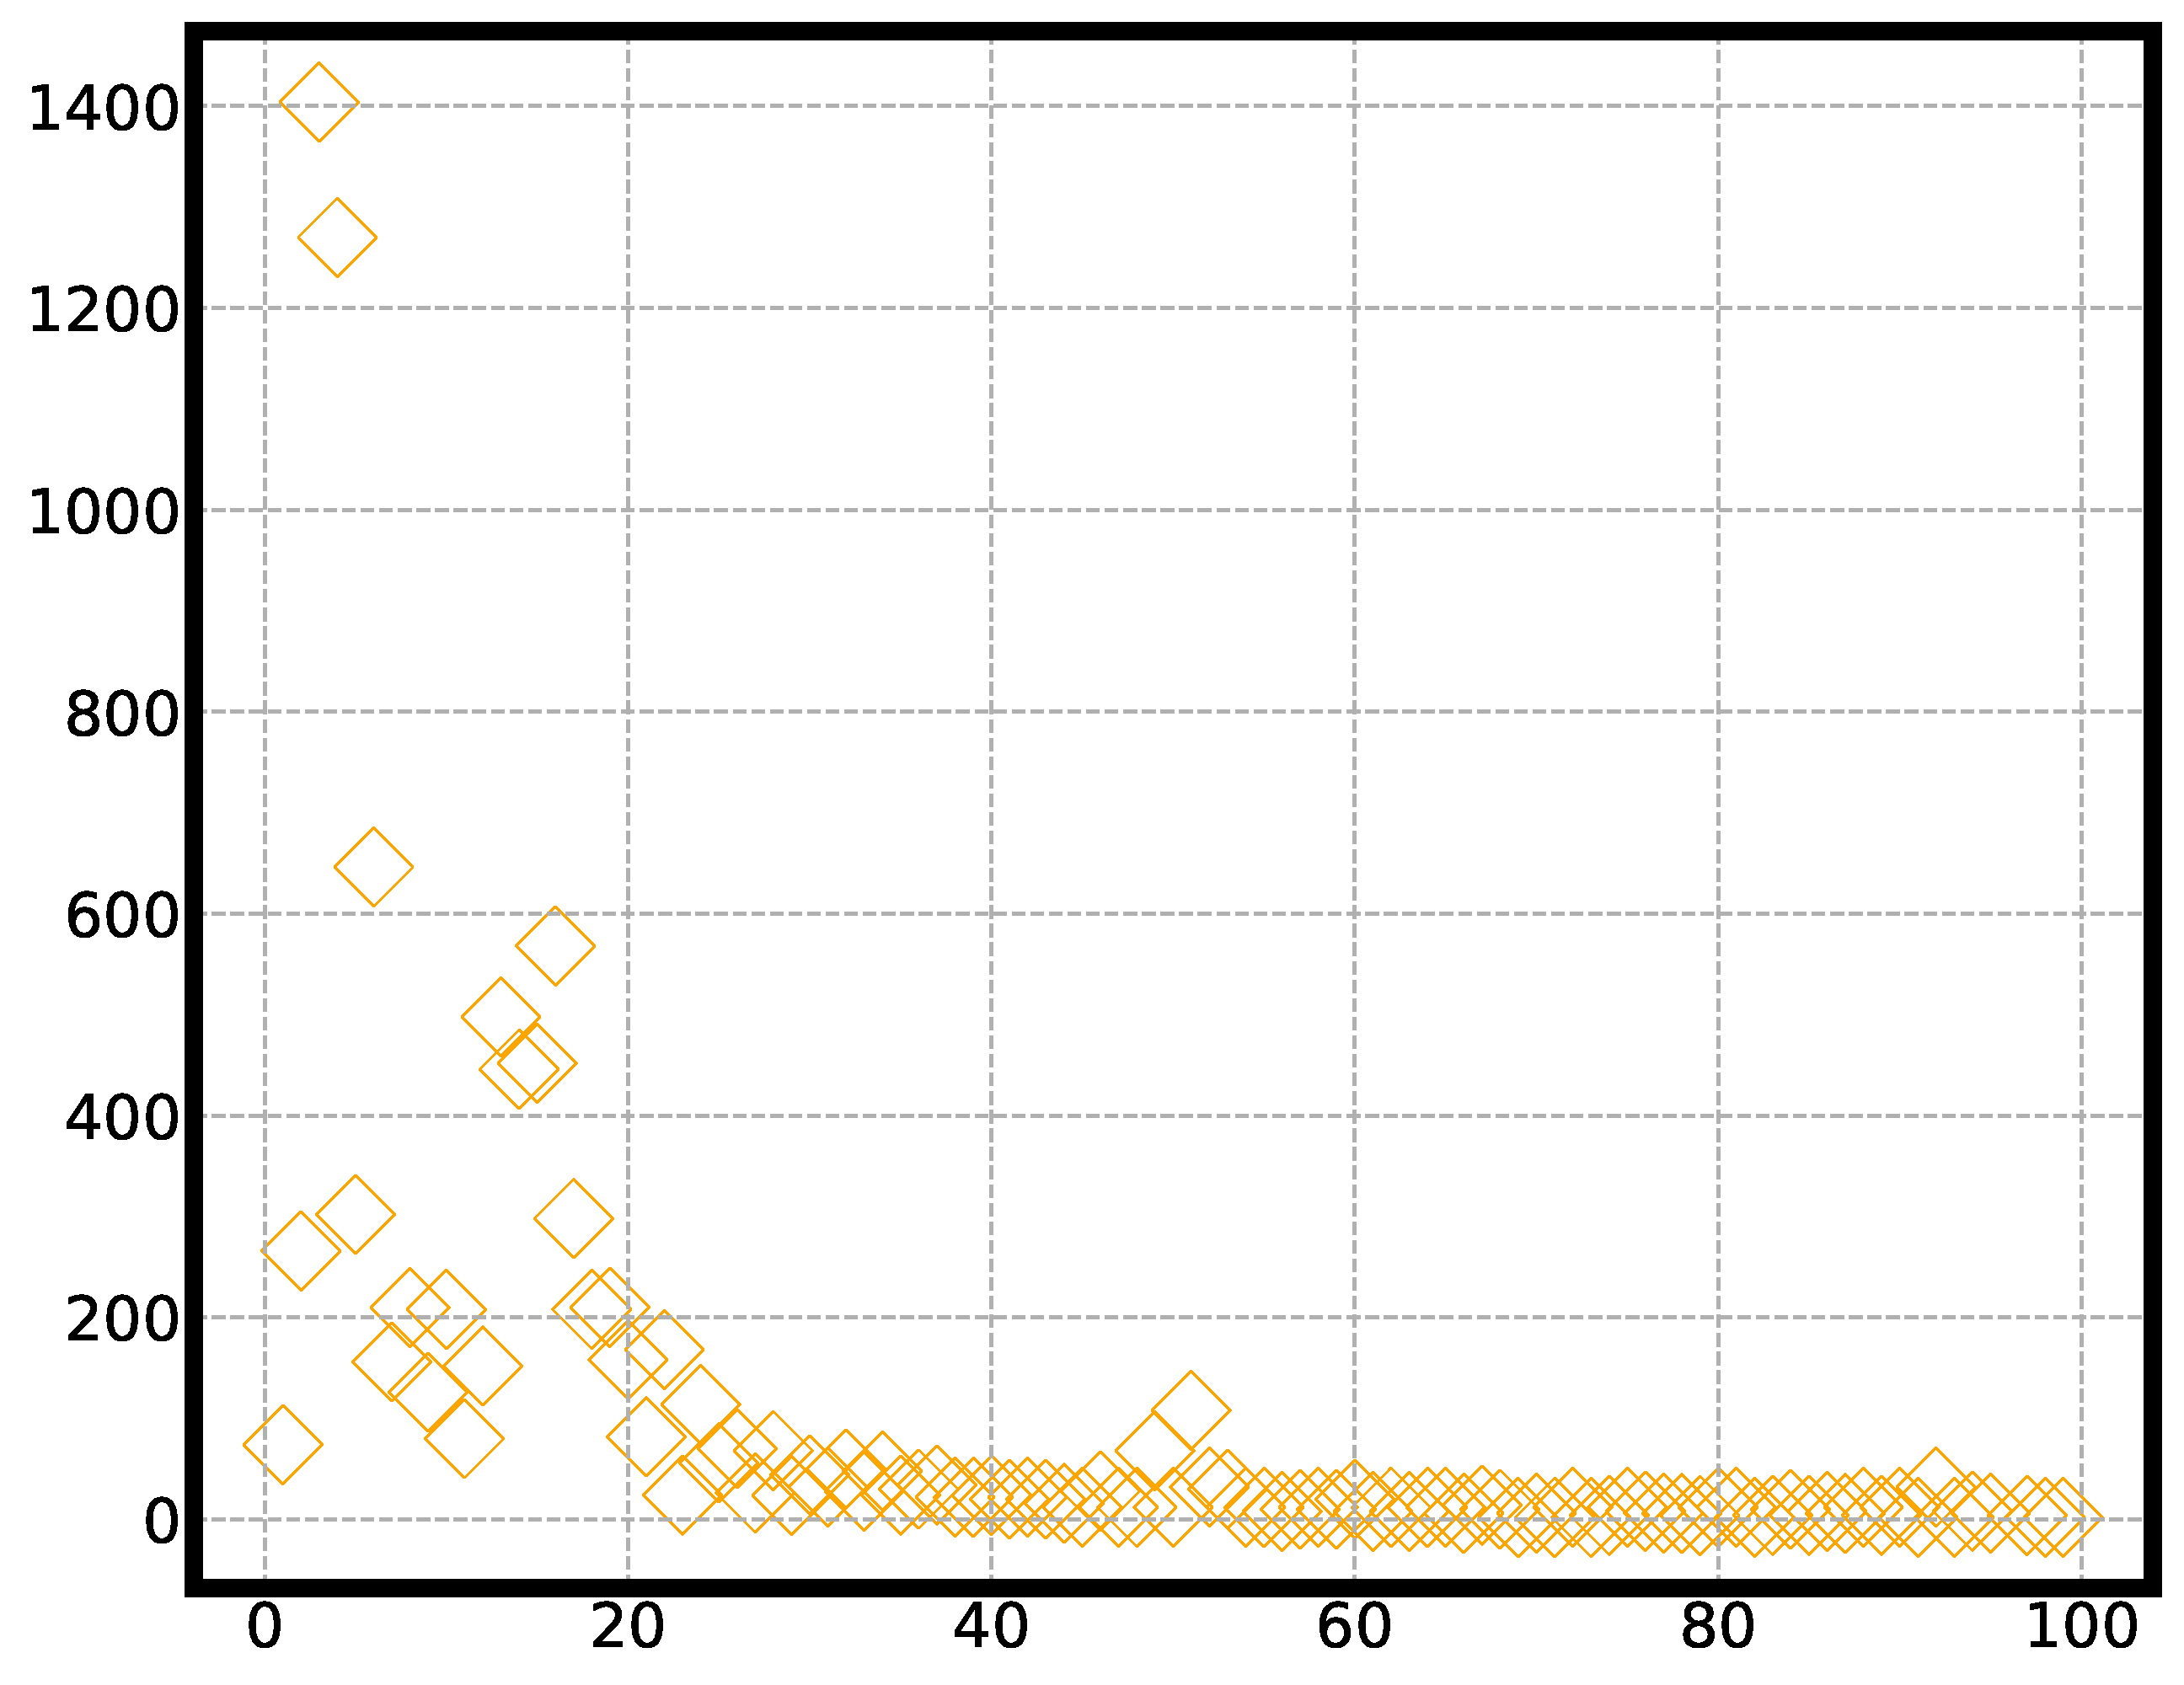
\includegraphics[width=\textwidth]{jinritoutiao-count.eps}
      \caption{}
      \label{fig:packet-size-jinritoutiao}
    \end{subfigure}%
    ~% add desired spacing
    \begin{subfigure}[b]{0.35\textwidth}
      \includegraphics[width=\textwidth]{cloudmusic-count.eps}
      \caption{}
      \label{fig:packet-size-netease-cloud-music}
    \end{subfigure}
    \bicaption{包大小特征。(a) 饿了么,(b) 美团,(c) 今日头条,(d) 网易云音乐。}{Packet Size.(a)Ele , (b)Meituan , (c)Jinritoutiao , (d)Netease-cloud-music.}
    \label{fig:packet-size-eda}
\end{figure}





由于已经有了流程对象,因此可以转向流程的数字矢量表示。


\emph{(i)}对于PS视图,通过计算前16个数据包的大小(用-1填充),我们形成了$ 16 $维矢量$ v_ {ps} $。

\emph{(ii)}\citep{wiana2019}对于CT视图,我们通过将值内容类型字段扩展为前16个数据包(用-1填充)来形成$ 16 $维矢量$ v_ {ct} $,其范围从0到255 。

\emph{(iii)}对于PB视图,通过将有效载荷字节值视为相应的ASCII码,我们形成一个$ 16 \ times64 = 1024 $维向量$v_{pb}$,然后进一步转换为0-255( 用-1填充)。





\subsection{多视图特征}
模型中包含了三个视图,分别称为数据包大小(PS)视图,数据包内容类型(CT)视图和数据包有效载荷字节(PB)视图。


\begin{itemize}

	\item \textbf{从 PB 提取特征:} 
	%
	我们使用一维卷积神经网络处理 $v_{pb}$向量。
	%
	在处理过程中, 使用了两层卷积神经网络, 每一层卷积的卷积核数量是 64, 卷积核的大小是$1 \times 3$, 卷积操作中我们采用的是max pooling。 
	%
	原始的payload部分的转换为64维的向量 $\alpha$.
	%
	\begin{equation}
		\alpha = \mathit{1\!D\!-\!C\!N\!N}(v_{pb})
	\end{equation}

	\item \textbf{从PS视图提取特征:}
	%
	$v_{ps}$向量和处理payload部分的一样,使用一维卷积神经网络进行处理, 所不同的是输入的向量大小为packet的数目。
	%
	经过一维卷积神经网络的处理后, packet size 序列被转换为一个64维的向量 $\beta$.
	%
	\begin{equation}
		\beta = \mathit{1D\!-\!C\!N\!N}(v_{ps})
	\end{equation}
	%
	\item \textbf{从CT视图提取特征:} 
	%
	content type 是一个用257维的one-hot编码的稀疏向量,每一个取值之间的距离为$\sqrt{2}$,one-hot夫人编码方式不能够有效表示上下文关系, 所以我们引入了embedding操作将这个257维的稀疏表示映射为一个16维的实数向量,这种表示方法有效保留了上下文关系。
	%
	Embedding层需要学习一个转换向量,其大小为 $ (vocab\_size, embedding\_dim) $.
	%
	The embedding layer is basically a matrix which can be considered a transformation from discrete and sparse 1-hot-vector into a continuous and dense latent space. 
	
	经过Embedding操作后,我们使用了循环神经网络从CT视图序列特征中提取抽象特征,形式上, 
	\begin{equation}
		\gamma = \mathit{R\!N\!N}(Embedding(v_{ct}))
	\end{equation}
	
	经过RNN处理后,content type视图被转换为一个64维的向量$\gamma$
	
\end{itemize}






\subsection{识别模块}
%
将三个不同的抽象特征连接在一起以形成192维向量。
% 
\begin{equation}
	\delta = \alpha \oplus \beta \oplus \gamma
\end{equation}
%
然后将其输入到完全连接的层。
\begin{table}[!htbp]
    \bicaption{AIBMF网络}{AIBMF network.}
    \label{tab:AIBMF-layer}
    \centering
    \footnotesize% fontsize
    \setlength{\tabcolsep}{4pt}% column separation
    \renewcommand{\arraystretch}{1.2}%row space 
    \begin{tabular}{|c|c|c|c|}
        \hline
        \textbf{网络层(类型)} & \textbf{输出层} & \textbf{参数个数} & \textbf{上一层网络}\\
        \hline
        \hline
        packetPayload (InputLayer) & (None, 1024) & 0 & \\
        \hline
        packetSize (InputLayer) & (None, 16) & 0 & \\
        \hline
        batch\_normalization\_1 (BatchNor) & (None, 1024) & 4096 & packetPayload[0][0] \\
        \hline
        batch\_normalization\_2 (BatchNor) & (None, 16) & 64 & packetSize[0][0] \\     
        \hline
        reshape\_1 (Reshape) & (None, 1024, 1) & 0 & batch\_normalization\_1[0][0] \\
        \hline
        reshape\_2 (Reshape) & (None, 16, 1) & 0 & batch\_normalization\_2[0][0] \\
        \hline
        layer\_conv\_1 (Conv1D) & (None, 1022, 64) & 256 & reshape\_1[0][0] \\
        \hline
        layer\_conv\_3 (Conv1D) & (None, 14, 64) & 256 & reshape\_2[0][0] \\
        \hline
        max\_pooling1d\_1 (MaxPooling1D) &  (None, 1020, 64) & 0 & layer\_conv\_1[0][0] \\ 
        \hline
        max\_pooling1d\_3 (MaxPooling1D) & (None, 12, 64) & 0 & layer\_conv\_3[0][0] \\
        \hline
        layer\_conv\_2 (Conv1D) & (None, 1020, 32) & 6176 & max\_pooling1d\_1[0][0] \\  
        \hline
        recordTypes (InputLayer) & (None, 16) & 0 & \\     
        \hline
        layer\_conv\_4 (Conv1D) & (None, 12, 32) & 6176 & max\_pooling1d\_3[0][0] \\
        \hline
        max\_pooling1d\_2 (MaxPooling1D) & (None, 1018, 32) & 0 & layer\_conv\_2[0][0] \\
        \hline
        embedding\_1 (Embedding) & (None, 16, 32) & 8224 & recordTypes[0][0] \\
        \hline
        max\_pooling1d\_4 (MaxPooling1D) &  (None, 10, 32) & 0 & layer\_conv\_4[0][0] \\
        \hline
        flatten\_1 (Flatten) & (None, 32576) & 0 & max\_pooling1d\_2[0][0] \\
        \hline
        lstm\_1 (LSTM) & (None, 16) & 3136 & embedding\_1[0][0] \\
        \hline
        flatten\_2 (Flatten) & (None, 320) & 0 & max\_pooling1d\_4[0][0] \\ 
        \hline
        dense\_1 (Dense) & (None, 64) & 2084928 & flatten\_1[0][0] \\
        \hline
        dense\_2 (Dense) & (None, 64) & 1088 & lstm\_1[0][0] \\
        \hline
        dense\_3 (Dense) & (None, 64) & 20544 & flatten\_2[0][0] \\
        \hline
        concatenate\_1 (Concatenate) & (None, 192) & 0 & dense\_1[0][0],dense\_2[0][0],dense\_3[0][0] \\
        \hline
        main\_output (Dense) & (None, 20) & 3860 & concatenate\_1[0][0] \\
        \hline
        \hline
        \textbf{总共参数} & \multicolumn{3}{|c|}{2,138,804} \\
        \textbf{可训练的参数} & \multicolumn{3}{|c|}{2,136,724} \\
        \textbf{不可训练的参数} & \multicolumn{3}{|c|}{2,080} \\
        \hline
    \end{tabular}
\end{table}

%
完全连接层的输出\emph {i.e。},$ x $,将用作softmax回归的输入,以识别流量。

三种不同的抽象特征共同优化同一类别目标,共同计算多类交叉熵损失,并通过反向传播算法更新三个神经网络的参数\cite{rumelhart1986learning}.
%
Mathematically, the probability that an output prediction $Y$ is app $a_j$, is determined by: 
\begin{equation}
p(Y=j|x,W,b)=\mathit{softmax_j}(\emph{\textbf{W}}x + \emph{\textbf{b}})
% =\frac{e^{w_i^TZ+b_i}}{\sum_je^{w_j^TZ+b_j}}
\end{equation}
where $W$ is a weight matrix between the fully connected layer and the softmax layer, and the $b$ is the bais vector.
% 
Then the model's prediction $y_{pd} $ is the class whose probability is maximal:
%
\begin{equation}
%
y_{pd}=argmax(p(Y=j|x,W,b)),\forall j \in \{1,2,3,...,C\}
\end{equation} 
%
我们的模型使用交叉熵 \citep{Boer2005A} 作为损失函数。 
%

\section{实验和评估}
\subsection{评估标准}
为了对AIBMF在交通数据上的识别性能进行合理有效的定量评估,本文介绍了一些基本指标:真阳性(TP),假阴性(FN),真阴性(TN)和假阳性( FP)。 TP是分类为应用程序$ i $的流量确切属于应用程序$ i $的数量。 FN是分类为应用程序$ i $的流数,完全属于应用程序$ j $。 TN是分类为应用程序$ j $的流数,完全属于应用程序$ i $。 FP是分类为应用程序$ j $的流数,完全属于应用程序$ j $。

请见表~\ref{tab:confusion-matrix}。
\begin{table}[!htbp]
    \bicaption{识别结果的混淆矩阵。}{Confusion matrix of classification results.}
    \label{tab:confusion-matrix}
    \centering
    \footnotesize% fontsize
    \setlength{\tabcolsep}{4pt}% column separation
    \renewcommand{\arraystretch}{1.2}%row space 
    \begin{tabular}{l|l|c|c|c}
        \multicolumn{2}{c}{}&\multicolumn{2}{c}{\textbf{预测结果}}&\\
        \cline{3-4}
        \multicolumn{2}{c|}{} & \textbf{正类} & \textbf{负类} & \multicolumn{1}{c}{\textbf{总计}}\\
        \cline{2-4}
        \multirow{2}{*}{\textbf{真实情况}} & \textbf{正类} & 真正类(TP) & 假负类(FN) & $TP+FN$\\
        \cline{2-4}
        & \textbf{负类} & 假正类(FP) & 真负类(TN) & $FP+TN$\\
        \cline{2-4}
        \multicolumn{1}{c}{} & \multicolumn{1}{c} {\textbf{总计}} & \multicolumn{1}{c}{$TP+FP$} & \multicolumn{    1}{c}{$FN+TN$} & \multicolumn{1}{c}{$TP+FN+FP+TN$}\\
    \end{tabular}
\end{table}



在训练阶段,\ emph {Accuracy(ACC)}用于指示模型识别能力的提高,并且改进了综合显示模型在识别HTTPS流量方面的性能。 准确率是在迭代训练过程中所有正确样本量与训练数据的比率,该比率是根据公式(7)计算的。


% ===========
% EQUATION:06
% ===========
\begin{equation}
ACC=\frac{TP+TN}{TP+TN+FP+FN}	
\end{equation}

在测试阶段,\ emph {Precision(P)}显示预测到应用程序$ i $的流量是实际应用程序$ i $,\ emph {Recall(R)}显示预测正确的流量与 属于应用程序$ i $的所有流,以及HTTPS流量的综合评估索引\ emph {F1}值都用作评估标准。 \ emph {P}根据公式(8a)计算; \ emph {R}根据公式(9a)计算; F1值是结合两个指标的综合评价指标,是根据公式(10a)计算的。 为了在所有20个应用程序上评估我们的方法,我们将平均值$ P $,$ R $,$ F_1 $ --- $ Macro \ Precision $,$ Macro \ Recall $,$ Macro \ F_1 $作为整体指标 式(8b),(9b),(10b)。 


% ===========
% EQUATION:07
\begin{subequations}
	\begin{equation}
	P=\frac{TP}{TP+FP}
	\end{equation}
	
	\begin{equation}
	Macro\ Precision=\frac{1}{20}\sum_{i=1}^{20}P_i
	\end{equation}
	
\end{subequations}

% ===========
% EQUATION:08
% ===========
\begin{subequations}
	\begin{equation}
	R=\frac{TP}{TP+FN}	
	\end{equation}
	
	\begin{equation}
	Macro\ Recall=\frac{1}{20}\sum_{i=1}^{20}R_i
	\end{equation}
\end{subequations}


% ===========
% EQUATION:09
% ===========
\begin{subequations}
	\begin{equation}
	F_1=2\frac{P\times R}{P+R}
	\end{equation}
	
	\begin{equation}
	Macro\ F_1=\frac{1}{20}\sum_{i=1}^{20}F_{1i}
	\end{equation}
\end{subequations}


\subsection{实验环境和数据集的组织}

请见表~\ref{tab:experiment-enviorment}。
\begin{table}[!htbp]
    \bicaption{实验所需的软硬件环境。}{Hardware and software environment of experiments.}
    \label{tab:experiment-enviorment}
    \centering
    \footnotesize% fontsize
    \setlength{\tabcolsep}{4pt}% column separation
    \renewcommand{\arraystretch}{1.2}%row space 
    \begin{tabular}{lcc}
        \hline
        \multirow{3}{*}{硬件} & CPU & 24 Intel (R) Xeon CPU E5-2650 v4 @ 2.2GHz \\
        & GPU & 2 GTX TITAN X \\
        & RAM & 128GB\\
        \hline
        \multirow{5}{*}{软件} & 操作系统 & Ubuntu 16.04 LTS\\
        & 编程语言 & Python 3.6, Linux bash \\
        & 深度学习框架 & Tensorflow 1.12,Keras 2.2.4\\
        & 机器学习框架 & scikit-learn 0.22.1\footnote{https://scikit-learn.org/}\\
        & 重要Python包 & Scapy\footnote{https://scapy.net/}, Pandas\footnote{https://pandas.pydata.org/}, Numpy\footnote{https://numpy.org/}, Matplotlib\footnote{https://matplotlib.org/} \\
        \hline
    \end{tabular}
\end{table}


我们将100,000+个带有标签的示例分为两个部分:训练集和测试集。 为了确保随机性,我们对数据进行了随机操作,其中训练集占90%,测试集占10%。


\subsection{超参数的确定}

\subsubsection{单个样本packet数目确定}
我们收集了100,000多个流数据,并研究了各种应用程序的数据包计数分布。如图4所示,超过100,000个流的数据包计数的中位数为11,一个流中的数据包计数超过16只占32%,我们将每一个packet的payload部分暂时定为16个字节,针对每一条流,取用不同的packet的数目进行对比实验,发现,随着packet的数目的增加,我们的模型的识别效果也在持续增加,当packet的数目增加为16个的时候,识别的效果不再由明显的变化,但是经过分析,随着packet数目的增加,模型所需要的空间复杂度和时间复杂度都会增加。在这里,将packet的数目取为16.
% =================================
% Fig. 03: Model architecture
% =================================
\begin{figure}[!htbp]
    \centering
    \begin{subfigure}[b]{0.45\textwidth}
      \includegraphics[width=\textwidth]{Packet-count-all.eps}
      \caption{}
      \label{fig:oaspl_a}
    \end{subfigure}%
    ~% add desired spacing
    \begin{subfigure}[b]{0.45\textwidth}
      \includegraphics[width=\textwidth]{Packet-count-acc.eps}
      \caption{}
      \label{fig:oaspl_b}
    \end{subfigure}
    ~% add desired spacing

    \bicaption{总声压级。(a) 这是子图说明信息,(b) 这是子图说明信息。}{OASPL.(a) This is the explanation of subfig, (b) This is the explanation of subfig.}
    \label{fig:oaspl}
\end{figure}


\subsubsection{单个packet的payload字节数确定}
为了确定每个数据包使用多少字节,我们进行了一系列比较实验。如图5所示,每个数据包以不同的长度截取,随着截取长度的增加,1D-CNN的识别能力增强。 当采用前64个字节时,测试集的准确性为93.34%。在64个字节的长度之后,精度会非常缓慢地增加,并且增益随着长度的增加而降低,但是1D-CNN的时间复杂度和空间复杂度将显着增加,因此每个数据包的长度设置为64。

\begin{figure}[!htbp]
	\centering
	\includegraphics[width=0.80\textwidth]{Payload-size-acc.eps}
	\bicaption{packet size}{view comparation}
	\label{fig:payload size}
\end{figure}

\subsection{不同深度学习模型的评估}
在实验的过程种,我们分别比较了仅仅使用一维卷积神经网络、二维卷积神经网络处理payload视图和AIBMF模型训练的过程,对比了在识别的过程中,loss和accuracy的变化过程。
\begin{figure}[!htbp]
    \centering
    \begin{subfigure}[b]{0.45\textwidth}
      \includegraphics[width=\textwidth]{AIBMF-training-loss.png}
      \caption{}
      \label{fig:oaspl_a}
    \end{subfigure}%
    ~% add desired spacing
    \begin{subfigure}[b]{0.45\textwidth}
      \includegraphics[width=\textwidth]{AIBMF-training-acc.png}
      \caption{}
      \label{fig:oaspl_b}
    \end{subfigure}
    ~% add desired spacing

    \bicaption{总声压级。(a) 这是子图说明信息,(b) 这是子图说明信息。}{OASPL.(a) This is the explanation of subfig, (b) This is the explanation of subfig.}
    \label{fig:oaspl}
\end{figure}

\subsection{传统方法和研究方法的对比}
我们的研究工作还对比了机器学习的方法,首先使用特征工程的方法构建了23种特征,见表:\ref{tab:statistical-feature},其中7种特征是根据HTTPS协议定义的特征,属于HTTPS流量特有的特征,其余的16种特征是流量分析工作常用的特征。

\begin{table}[!htbp]
    \bicaption{统计特征。}{Statistical Feature.}
    \label{tab:statistical-feature}
    \centering
    \footnotesize% fontsize
    \setlength{\tabcolsep}{4pt}% column separation
    \renewcommand{\arraystretch}{1.2}%row space 
	\begin{tabular}{| c | c | c |}
		\hline
		\textbf{统计特征} & \textbf{含义} & \textbf{是否是HTTPS特有?}\\
		\hline
		\hline
		Packet counts & Packet数量& 否\\
		\hline
		TTL max & TTL最大值 & 否\\
		\hline
		TTL min & TTL最小值 & 否\\
		\hline
		TTL mean & TTL平均值 & 否\\
		\hline
		TTL median & TTL中位数 & 否\\
		\hline
		TTL var & TTL方差 & 否\\
		\hline
		packet\_length max & packet长度最大值 & 否\\
		\hline
		packet\_length min & packet长度最小值 & 否\\
		\hline
		packet\_length mean & packet长度平均值 & 否\\
		\hline
		packet\_length median & packet长度中位数 & 否\\
		\hline
		packet\_length var & packet长度方差 & 否\\
		\hline	
		window max & 窗口最大值 & 否\\
		\hline
		window min & 窗口最小值 & 否\\
		\hline
		window mean & 窗口平均值 & 否\\
		\hline
		window median & 窗口中位数 & 否\\
		\hline
		window var & 窗口方差 & 否\\
		\hline
		session\_id\_length max & session id长度 & 否\\
		\hline	
		client\_extensions\_length max & client extensions长度最大值 & 是\\
		\hline
		client\_extensions\_length min & client extensions长度最小值 & 是\\
		\hline
		client\_extensions\_length mean & client extensions长度平均值 & 是\\
		\hline
		client\_extensions\_length median & client extensions长度中位数 & 是\\
		\hline
		client\_extensions\_length var & client extensions长度方差 & 是\\
		\hline
		client\_ciphers counts & 客户端加密组件种类 & 是\\
		\hline
		server\_cipher & 服务端加密组建类型 & 是\\
		\hline
	\end{tabular}
\end{table}
针对提取的23种特征,分别使用了随机森林,支持向量机和单层神经网络进行训练和识别,如下表,和我们的研究工作提出的AIBMF模型相比较,基于机器学习的方法在识别能力表现不是很优秀。我们的AIBMF模型在三个参数上均领先于其他的识别模型。
\begin{table}
	\caption{traffic identification based on statistical features only}
	\begin{center}
		\begin{tabular}{|c||c||c||c|}
			\hline
			\textbf{Machine learning algorithm} & \textbf{Precision} & \textbf{Recall} & \textbf{F1} \\
			\hline
			\hline
			Random Forest & 0.8805 & 0.8172 & 0.8407 \\
			\hline
			SVM-RBF & 0.9214 & 0.5754 & 0.6676 \\
			\hline
			DNN & 0.7362 & 0.6293 & 0.6562 \\
			\hline
			\textbf{AIBMF} & \textbf{0.918} & \textbf{0.909} & \textbf{0.913} \\
			\hline
		\end{tabular}
		\label{tab4}
	\end{center}
\end{table}


\subsection{AIBMF模型识别效果}
针对20个移动应用1万条样本,绘制混淆矩阵来观察识别的效果。整体上,识别的效果非常好,其中大多数的错误是由于不同的应用之间可能共享服务所致,尤其针对那些由同一个公司开发的应用而言,识别能力存在一定的混淆。有一些应用将其API提供给了其他的应用作为公共接口,如百度地图,这给我们模型的识别能力带来了一定的影响。另外我们发现在我们的实验中,QQ软件的识别效果最差。 可能的原因是QQ使用的通信协议主要是UDP,并补充了TCP协议。 我们主要从Qzone捕获QQ流量,该流量混合了许多其他应用程序的流量。

\begin{figure}[!htbp]
	\centering
	\includegraphics[width=0.80\textwidth]{AIBMF-confusematrix.png}
	\bicaption{AIBMF识别混淆矩阵}{AIBMF classification confusematrix}
	\label{fig:AIBMF_confusematrix}
\end{figure}


\section{小结}
人工定义的统计特征越复杂,流量识别任务的通用性就越差。但是,仅使用深度学习忽略协议设计的信息来处理有效负载,识别能力也受到限制。实际上,协议定义的一些有意义的信息(例如内容类型)花费很少的精力,在流量分析中很有用。因此,从多个角度分析HTTPS流量并组合不同的功能可能是将来加密流量分析中的有力选择。本章节提出了一种通过HTTPS流量进行应用程序识别的方法-AIBMF。我们的方法能够分析HTTPS应用流量并将HTTPS流量与特定的移动应用相关联。
\chapter{基于增量学习的新移动应用识别方法}\label{chap:transfer}
\section{引言}
目前的加密流量识别方法具有一个主要缺点,那就是新应用程序继续遭受\textit{灾难性遗忘}\citep{french1999catastrophic,robins1995catastrophic,kirkpatrick2017overcoming}的困扰,当逐步增加新的应用程序类别进行培训时,整体性能会急剧下降。当前已有的研究工作均是需要全部的流量数据来训练,针对新出现的应用,需要将原来的流量数据和新来的应用的流量数据合并一起重新进行训练,当应用不断出现,训练的样本数量会急剧增加,这将给流量数据的存储以及模型的训练带来巨大的压力。为了解决这个问题,提出\emph{IncreAIBMF}框架,以使用新的应用程序数据以及仅对应于旧应用程序样本的一小样本集逐步学习深度神经网络。

为了验证我们提出的IncreAIBMF模型的优越性,在本章本章将IncreAIBMF模型分别和针对AIBMF模型微调、全量训练进行比较。



\section{方法描述}

\subsection{增量学习框架}
如图:\ref{fig:IncreAIBMF-architecture}所示,IncreAIBMF由三个模块构成:训练集构建,训练,代表性存储空间。
\begin{figure}[!htbp]
	\centering
	\includegraphics[width=0.95\textwidth]{IncreAIBMF.pdf}
	\bicaption{IncreAIBMF架构}{IncreAIBMF architecture}
	\label{fig:IncreAIBMF-architecture}
\end{figure}

分别介绍如下:
\subsubsection{构建训练集}
此阶段准备训练数据以用于下一个训练阶段。训练集由旧类的代表性样本的一部分(代表存储器中存储的旧类的示例)和新的app类的样本组成。由于我们的方法使用了两个损失函数,即分类和精馏,因此每个样本都需要两个标签,与这两个损失相关联。为了进行分类,我们使用one-hot向量来指示应用程序出现在所有应用程序类中。对于精馏,使用每个识别模块使用旧的应用程序类生成的精馏标签。因此,每个样品的蒸馏标签与具有旧应用程序类的识别模块一样多。此时,两个标识模块将在旧应用程序上运行,一个标识模块将处理新应用程序。对样品进行评估时,将使用旧应用程序的两个识别模块生成的精馏标签用于精馏,将使用三个识别模块生成的精馏标签用于分类。


\subsubsection{训练过程}
训练阶段将带有相应标签的增强训练集作为交叉蒸馏损失计算的输入,并更新整个网络体系结构的所有参数。 交叉蒸馏损失函数L定义如公式:(\ref{eqn:cdl})所示。
\begin{equation}
	\label{eqn:cdl}
	L(\omega)=L_{C}(\omega)+\lambda\sum_{f=1}^{F} L_{D_{f}}(\omega)
\end{equation}

这里 $L_{C}(\omega)$是应用于新旧类别样本的交叉熵损失。
%
$ L_{D_{f}} $是分类层$ f $的蒸馏损失,$ F $是旧应用程序的分类层总数。
%
$ \lambda $是指交叉蒸馏损失中蒸馏损失的比率。 在训练过程中,我们将其设置为0.3。
%
交叉熵损失$ L_{C}(\omega)$由下式给出:
%
\begin{equation}
	L_{C}(\omega)=-\frac{1}{N} \sum_{i=1}^{N} \sum_{j=1}^{C} p_{i j} \log q_{i j}
\end{equation}
%
其中$ qi $是通过对样本$ i $的分类层的logit应用softmax函数获得的分数,$ pi $是样本$ i $的基本事实,$ N $和$ C $表示 样本数和类别。
%
精馏损失 $L_{D}(\omega)$ 定义为:
%
\begin{equation}
	L_{D}(\omega)=-\frac{1}{N} \sum_{i=1}^{N} \sum_{j=1}^{C} { pdist }_{i j} \log {qd i s t}_{i j}
\end{equation}
%
其中$ pdisti $和$ qdisti $分别是$ pi $和$ qi $的修改版本。

\subsubsection{代表性空间更新}
此阶段的目标是更新内存中的样本,并确保训练集的大小不会急剧增加。也就是说,在更新的内存中,本章将内存大小固定为$ K $个流量(本文中$ K = 100,000 $),并且与每个应用程序类别相对应的样本数为$ \frac{100,000}{C} $,此处$ C $表示应用程序的类别。

然后,采用两个操作:

\begin{itemize}
    \item 选择要存储的新样本:执行herding采样\citep{welling2009herding},该策略根据与该类别的平均样本的距离生成一类样本的排序列表;给定样本的排序列表,选择列表中的前$ n $个样本。这些样本根据平均值最能代表该类别。
    \item 删除剩余的样本:由于样本存储在排序列表中,因此此操作很简单。存储单元仅需要从每个类别的样本集的末尾删除样本。请注意,执行此操作后,删除的样本将不再使用。 
\end{itemize}


\section{实验评估}

\subsection{微调效果}
面对越来越多的应用程序,常用的方法之一是微调。微调方法是指基于训练后的模型添加少量任务特定的参数。例如,对于分类问题,将softmax网络层添加到模型中,然后对新类进行重新训练以进行微调。对于新收集的30个应用程序的流量,本文首先使用微调的想法,冻结在20个旧应用程序上训练的AIBMF网络模型的参数以进行特征提取,并且仅修改完全连接的层数。在每个训练步骤添加$L \in \emph{[5,10,15,20,25,30]}$个应用。如图\ref {fig:AIBMF-Fine-tuning}所示,新模型无法完成旧类别和新类别中的识别任务,本文将这种糟糕的表现归因于灾难性的遗忘。迁移学习是一种处理新数据的有效方法,它普遍使用的场景为:原始模型是通过大量的数据训练得到的,处理的新数据是更为小范围的数据,即原始模型本身训练了更多的数据,具有更强的特征建模能力。在我们的研究过程中,应用不断出现,原始模型的数量要远远少于新增数据的数量,另外实验结果表明,微调的方法并不能够很好处理本研究课题面对的新增应用数量巨大带来的问题。

\begin{figure}[!htbp]
	\centering
	\includegraphics[width=0.45\textwidth]{AIBMF-Fine-tuning.pdf}
	\bicaption{AIBMF微调识别效果}{AIBMF Fine tuning}
	\label{fig:AIBMF-Fine-tuning}
\end{figure}

\subsection{增量学习效果}
本章使用第四章所训练的AIBMF模型筛选出原始的代表性空间,并将该空间的大小设置为10条样本,筛选的方法为通过该模型计算出全连接层的向量,计算出所有样本计算的全连接层向量的中心点,保留前$100000/K$的距离中心点最近的样本,在这里100000表示的是代表性空间的大小,$K$代表的是类别数目,如一开始$K=20$,则在构建代表性空间的时候,每一个应用被保留的样本的数量将会$\leq 5000$,即每一个应用距离中心点的前5000个样本会被保留,不够5000的将会被全部保留。本章使用的评估指标和实验环境与第四章相同。


为了验证基于增量学习的模型IncreAIBMF模型在所有50个应用20多万条流的样本上识别效果,本章首先使用第四章所述的AIBMF模型对50个应用一次性进行训练,其中18条流用于训练,2万多条流用于验证。

图:\ref{fig:Time-cost}对比了AIBMF模型和Increment模型在随着样本数量增加的时候训练所需要的时间变化情况。对于AIBMF模型,新应用增加的时候,模型需要重新对整个数据集进行训练,训练的样本的数量会持续增加,因此图中AIBMF模型的训练时间消耗随着应用的出现持续增加。而IncreAIBMF模型限制了训练集的规模,当新的应用出现的时候,训练集的规模并不会爆炸增加,因此图中IncreAIBMF模型的训练时间消耗随着新应用的出现变化不大。
\begin{figure}[!htbp]
	\centering
	\includegraphics[width=0.45\textwidth]{Time-cost-incre.eps}
	\bicaption{AIBMF和IncreAIBM时间消耗对比 }{Time cost comparation between AIBMF and IncreAIBMF}
	\label{fig:Time-cost}
\end{figure}

图:\ref{fig:AIBMF-IncreAIBMF}是AIBMF和IncreAIBMF模型在识别效果上的对比,共包含了精确度(Mpre)、Fi值(MF1)和召回率(Mrec)三个标准。其中图:\ref{fig:AIBMF-performance}是AIBMF在应用类别增加的时候的识别效果变化,可见AIBMF在应用类别增加的时候具备鲁棒性。图:\ref{fig:IncreAIBMF-performance}是IncreAIBMF模型在应用类别增加的时候的识别效果变化,和AIBMF相比,识别性能的差距很微弱,即IncreAIBMF模型保持了AIBMF的识别性能。
\begin{figure}[!htbp]
    \centering
    \begin{subfigure}[b]{0.45\textwidth}
      \includegraphics[width=\textwidth]{Full-comparation.eps}
      \caption{}
      \label{fig:AIBMF-performance}
    \end{subfigure}%
    ~% add desired spacing
    \begin{subfigure}[b]{0.45\textwidth}
      \includegraphics[width=\textwidth]{Incre-comparation.eps}
      \caption{}
      \label{fig:IncreAIBMF-performance}
    \end{subfigure}
    ~% add desired spacing
    \bicaption{AIBMF和IncreAIBMF识别效果对比。(a) AIBMF识别效果,(b) IncreAIBMF识别效果。}{Comparation of the Performance between AIBMF and IncreAIBMF.(a) AIBMF Performance, (b) IncreAIBMF Performance.}
    \label{fig:AIBMF-IncreAIBMF}
\end{figure}


图:\ref{fig:IncreAIBM-confuse-matrix}是IncreAIBMF模型在50个应用,2万余条样本上的识别效果。在大多数情况下,识别性能几乎是完美的,错误是依然是由于不同应用之间的网络服务共享所致,尤其是同一开发人员开发的应用(例如”闲鱼“和”阿里巴巴“均由AliBaBa.com开发,”闲鱼“被IncreAIBMF错误地识别为”阿里健康“)。另外”天涯“的用户量很少,检查了数据集的组成,发现”天涯“的样本很少(因为该应用不再活跃且大部分通信没有使用HTTPS协议),对其识别效果差是数据不均衡造成的。
\begin{figure}[!htbp]
	\centering
	\includegraphics[width=0.90\textwidth]{Incre-confuse-matrix.pdf}
	\bicaption{IncreAIBM 识别混淆矩阵}{IncreAIBM confuse matrix}
	\label{fig:IncreAIBM-confuse-matrix}
\end{figure}



\section{本章小节}
这一部分提出了IncreAIBMF模型,有效处理新增应用的流量数据的识别,使得我们的识别模型能够有效克服灾难遗忘问题,在新增应用的识别任务上,能够有效节约时间和空间,更加高效完成识别任务。
\chapter{总结与展望}\label{chap:conclusion}
本章对论文工作和取得的成果进行总结,并展望后续基于HTTPS流量的移动应用识别任务中需要继续研究的新的研究课题。

\section{总结}
本文的研究目的是研究一种能够准确对移动应用HTTPS流量进行识别的方法,减少对复杂的特征工程的依赖,提高移动应用识别的性能。为此提出了基于多视图特征的移动应用HTTPS流量识别方法,在这个方法的基础之上,考虑到实际的应用场景,即移动应用新增以及更新迅速,提出了基于增量学习的新增移动应用识别方法。本文的主要工作在于:

1. 提出了自动化移动应用HTTPS流量标记方法,并抓取50个移动应用,20多万条流的HTTPS流量数据,解决当前所公布的开源数据较少、数据量有限、流量数据标记较为粗糙的问题,为本文后续的研究工作提供了可靠的有标记的实验数据集。

2. 提出了基于多视图特征的移动应用识别方法,首次从多个视图角度对HTTPS流量进行特征建模形成多视图特征,并在此基础上使用深度学习模型进行高阶特征学习和融合,最后完成移动应用识别任务。解决了现有的移动应用识别方法特征建模难、特征建模能力弱、识别模型受网络环境影响高的问题。

3. 提出了基于增量学习的新增移动应用识别方法,借助增量学习思想,利用新增流量数据和代表性流量样本共同训练识别模型,解决新应用不断涌现带来的因为灾难遗忘是的模型无法有效识别的问题,在真实的应用场景中对处理新增应用流量识别问题具有重要的实用价值。

\section{展望}
综上讨论,本文认为今后的研究工作可以从以下几个方面展开。

1. 为了采集更高质量的流量数据,可以针对流量的采集工作进行进一步的研究。本文在采集数据时是通过遍历移动应用中的事件产生随机事件产生流量进行捕获的,可以研究使用深度学习、强化学习驱动应用的运行,借助自动化测试领域的相关研究工作,对于流量数据采集具有重要的意义,可以更加贴近用户的使用习惯产生应用流量。

2. 本文中提出的识别模型中使用到的HTTPS协议定义的参数只包括内容类型(Content Type),可以探索更多的协议定义的参数在流量精细化识别工作中的价值,结合HTTPS协议和深度学习的方法在流量精细化识别任务上具有很广的探究前景。


%---------------------------------------------------------------------------